% Create a Table of Contents in Beamer
\documentclass[10pt,t]{beamer}
% Theme choice:
\usetheme{Singapore}
\useoutertheme{sidebar}
\usecolortheme{seahorse}
\setbeamercolor{titlelike}{bg=white}
\setbeamercolor{frametitle}{bg=white}
%\setbeamertemplate{frametitle}[default][left]
\setbeamertemplate{navigation symbols}{}
\setbeamertemplate{footline}{\begin{flushright}\small \insertframenumber\end{flushright}}

\usepackage{graphicx}
\usepackage{amsmath}
\usepackage{amsfonts}
\usepackage{amssymb}
\usepackage{amsthm}
\usepackage{ulem}
\usepackage{listings}

% Title page details: 
\title{Chapter 3: Prediction in Linear Regression} 
\author{Nina Galanter}
\date{\today}


\begin{document}
	% Title page frame
	\begin{frame}
	\titlepage 
\end{frame}

\begin{frame}{Learning objectives}
By the end of Chapter 3, you should be able to:

\vspace{0.3cm} 
\begin{itemize}
	\item Understand and explain the difference between the scientific goals of prediction vs. inference
	\medskip
	\item Be able to compute fitted values in \texttt{R} and by hand
		\medskip
	\item Understand the importance of training vs. testing data, and how to create training and testing datasets in \texttt{R}
		\medskip
	\item Determine the predictive accuracy of a linear regression analysis using $R^2$ and mean squared error (MSE)
		\medskip
	\item Use $R^2$ and MSE to choose a prediction model
\end{itemize}
\end{frame}

% Outline frame
\begin{frame}{Outline}
\tableofcontents
\end{frame}

\AtBeginSection[ ]
{
\begin{frame}{Outline}
\tableofcontents[currentsection]
\end{frame}
}

% Presentation structure
% Prediction vs. Inference - difference in goals
% Fitted values review & examples - in R and by hand
% Training and testing data
% Measures of prediction accuracy
% - R^2
% - MSE
% Bias-variance tradeoff


\section{Prediction vs. Inference}

\begin{frame}{Prediction vs. Inference}
So far in this course, our goal has been to estimate the association between a predictor of interest and our outcome.

\vspace{0.3cm}

In Chapter 2, we discussed the potential need to adjust for additional variables in our regression model (confounders, precision variables, effect modifiers). The inclusion of additional variables was motivated by scientific questions about  \textcolor{blue}{association}, which led us to conduct  \textcolor{blue}{statistical inference}.

\vspace{0.3cm}

When our scientific question involves  \textcolor{blue}{prediction}, we have a different goal in mind: develop an algorithm based on current data that, when we plug in future data, predicts the outcome well.
\end{frame}

\begin{frame}{Prediction vs. Inference}
In loose terms:
\vspace{0.3cm}

\textcolor{blue}{Prediction:} using a model to predict outcomes for new data points

\vspace{0.3cm}

\textcolor{blue}{Inference:} understanding the relationships between variables (typically a predictor of interest and an outcome)
\end{frame}

\begin{frame}{Inference: scientific questions}
With inference, we are able to answer questions such as\dots

\vspace{0.3cm}

\begin{itemize}
	\item Are individuals with a specific genetic variable more susceptible to certain diseases later in life?
	\medskip
	
	\item Is there an association between access to antenatal clinics and maternal mortality in rural areas?
	
	\medskip
	
	\item Was a certain public health intervention associated with improved health outcomes for a community?
	\medskip
	
	\item Is a new vaccine effective at reducing the risk of getting a disease, or perhaps a severe case of the disease?
\end{itemize}

\end{frame}

\begin{frame}{Prediction: scientific questions}
With prediction, we are instead interested in questions such as\dots

\vspace{0.3cm}

\begin{itemize}
	\item How do we predict risk of type II diabetes based on an individual's medical history?
	\medskip
	
	\item Can we accurately classify tumors in the central nervous system?
	
	\medskip
	
	\item What is the under-5 mortality rate at the state level for a country where we have no reliable census or vital registration data?
	\medskip
	
	\item Based on the videos a person has watched on YouTube, can we give them accurate suggestions for videos they would like to watch next?
\end{itemize}

\vspace{0.3cm}

* Questions like the last one are asked by companies all the time, including YouTube, TikTok, Netflix, or any company that provides some form of media or involves targeted advertising. 
\end{frame}




\begin{frame}{\textcolor{violet}{Pollev:} Prediction Intuition}
	
	We have 50 patients. We take white blood cell count measurements for each patient. The average count is 10,000 cells per microliter, with a standard deviation of 1000 cells per microliter. A new patient comes in from the exact same population. What is our best guess at what their white blood cell count will be?
	\smallskip
	
	\url{https://PollEv.com/multiple_choice_polls/cH0UFVJsBHbW9EULODiqT/respond}
	\pause
	
	\bigskip
	
	\textcolor{blue}{10,000 cells per microliter}
	
	
\end{frame}

\begin{frame}{\textcolor{violet}{Pollev:} Prediction Intuition}
	\vspace{-5 mm}
	Now we have slightly more information:
	
	\medskip
	
	We have 50 patients. We take white blood cell count measurements for each patient. 25 of the patients have the flu and 25 do not. 
	
	\medskip
	
	The average white blood cell count for patients with the flu is 15,000 cells per microliter, with a standard deviation of 1,000 cells per microliter.
	\medskip
	
	The average white blood cell count for patients without the flu is 5,000 cells per microliter, with a standard deviation of 1,000 cells per microliter.
	\medskip
	
	A new patient comes in from the exact same population. They have the flu What is our best guess at what their white blood cell count will be?
	
		\smallskip
	
	\url{https://PollEv.com/multiple_choice_polls/4pYsYukH1hi5w761GIrUa/respond}
	\pause
	
	\bigskip
	
	\textcolor{blue}{15,000 cells per microliter}
	
	
\end{frame}

\begin{frame}{Prediction Intuition}
	
	Restating the problem:
	
	\medskip
	
	We have 50 patients. We take white blood cell count measurements for each patient and also measure whether each has the flu. We use flu status to predict white blood cell count. We get the following regression equation:
	
	\medskip
	
\textcolor{blue}{	\[E[\text{Cell Count}|\text{Flu}]=5000+10000*\text{Flu}\]}
	\medskip
	
	A new patient comes in from the exact same population. They have the flu What is our best guess at what their white blood cell count will be?
	
	\bigskip
	
	\textcolor{blue}{15,000 cells per microliter}
	
	
\end{frame}

\section{Fitted values}

\begin{frame}{Fitted values}
	
	\vspace{-5 mm}
	
	How do we actually use a model to  \textcolor{blue}{predict} something? We use fitted values!
	
	\vspace{0.3cm}
	
	From Chapter 1:
	
	\vspace{0.3cm}
	
	\textbf{\textcolor{blue}{Fitted value}: the value of the response predicted from your regression}
	
	\vspace{0.3cm}
	
	Consider the linear regression model
	$$
	E[Y \mid X_1, \dots, X_p] = \beta_0 + \beta_1 X_1 + \dots + \beta_p X_p
	$$
	\smallskip
	
	If we fit this model, we obtain coefficient estimates $\hat{\beta}_0, \dots \hat{\beta}_p$, and we can plug them into our regression equation to get a fitted value $\hat{Y}$:
	
	\medskip
	$$
	\hat{Y} = \hat{\beta}_0 + \hat{\beta}_1 X_1 + \dots + \hat{\beta}_p X_p
	$$
	
	
\end{frame}

\begin{frame}{Fitted values}
Each observation in our dataset gets a fitted value, based on their covariates values $X_1, \dots, X_p$. If we denote each observation by $i = 1, \dots, n$ for $n$ total observations, the fitted value for observation $i$ is:
\medskip

$$
\hat{Y}_i = \hat{\beta}_0 + \hat{\beta}_1 X_{i, 1} + \dots + \hat{\beta}_p X_{i, p}
$$

\medskip

\begin{itemize}
\item Easy to visualize fitted values in two dimensions
\medskip

\item More difficult to visualize in more than two dimensions
\medskip

\item \textcolor{blue}{Fitted values  are the predicted values (predictions) for each observation in our dataset!}
\end{itemize}
\end{frame}

%\begin{frame}{Fitted values: Visualizing in two dimensions}
%In two dimensions (where we have only one predictor $X_1$), we can visualize fitted values on a scatter plot:
%\vspace{0.3cm}
%
%\centering 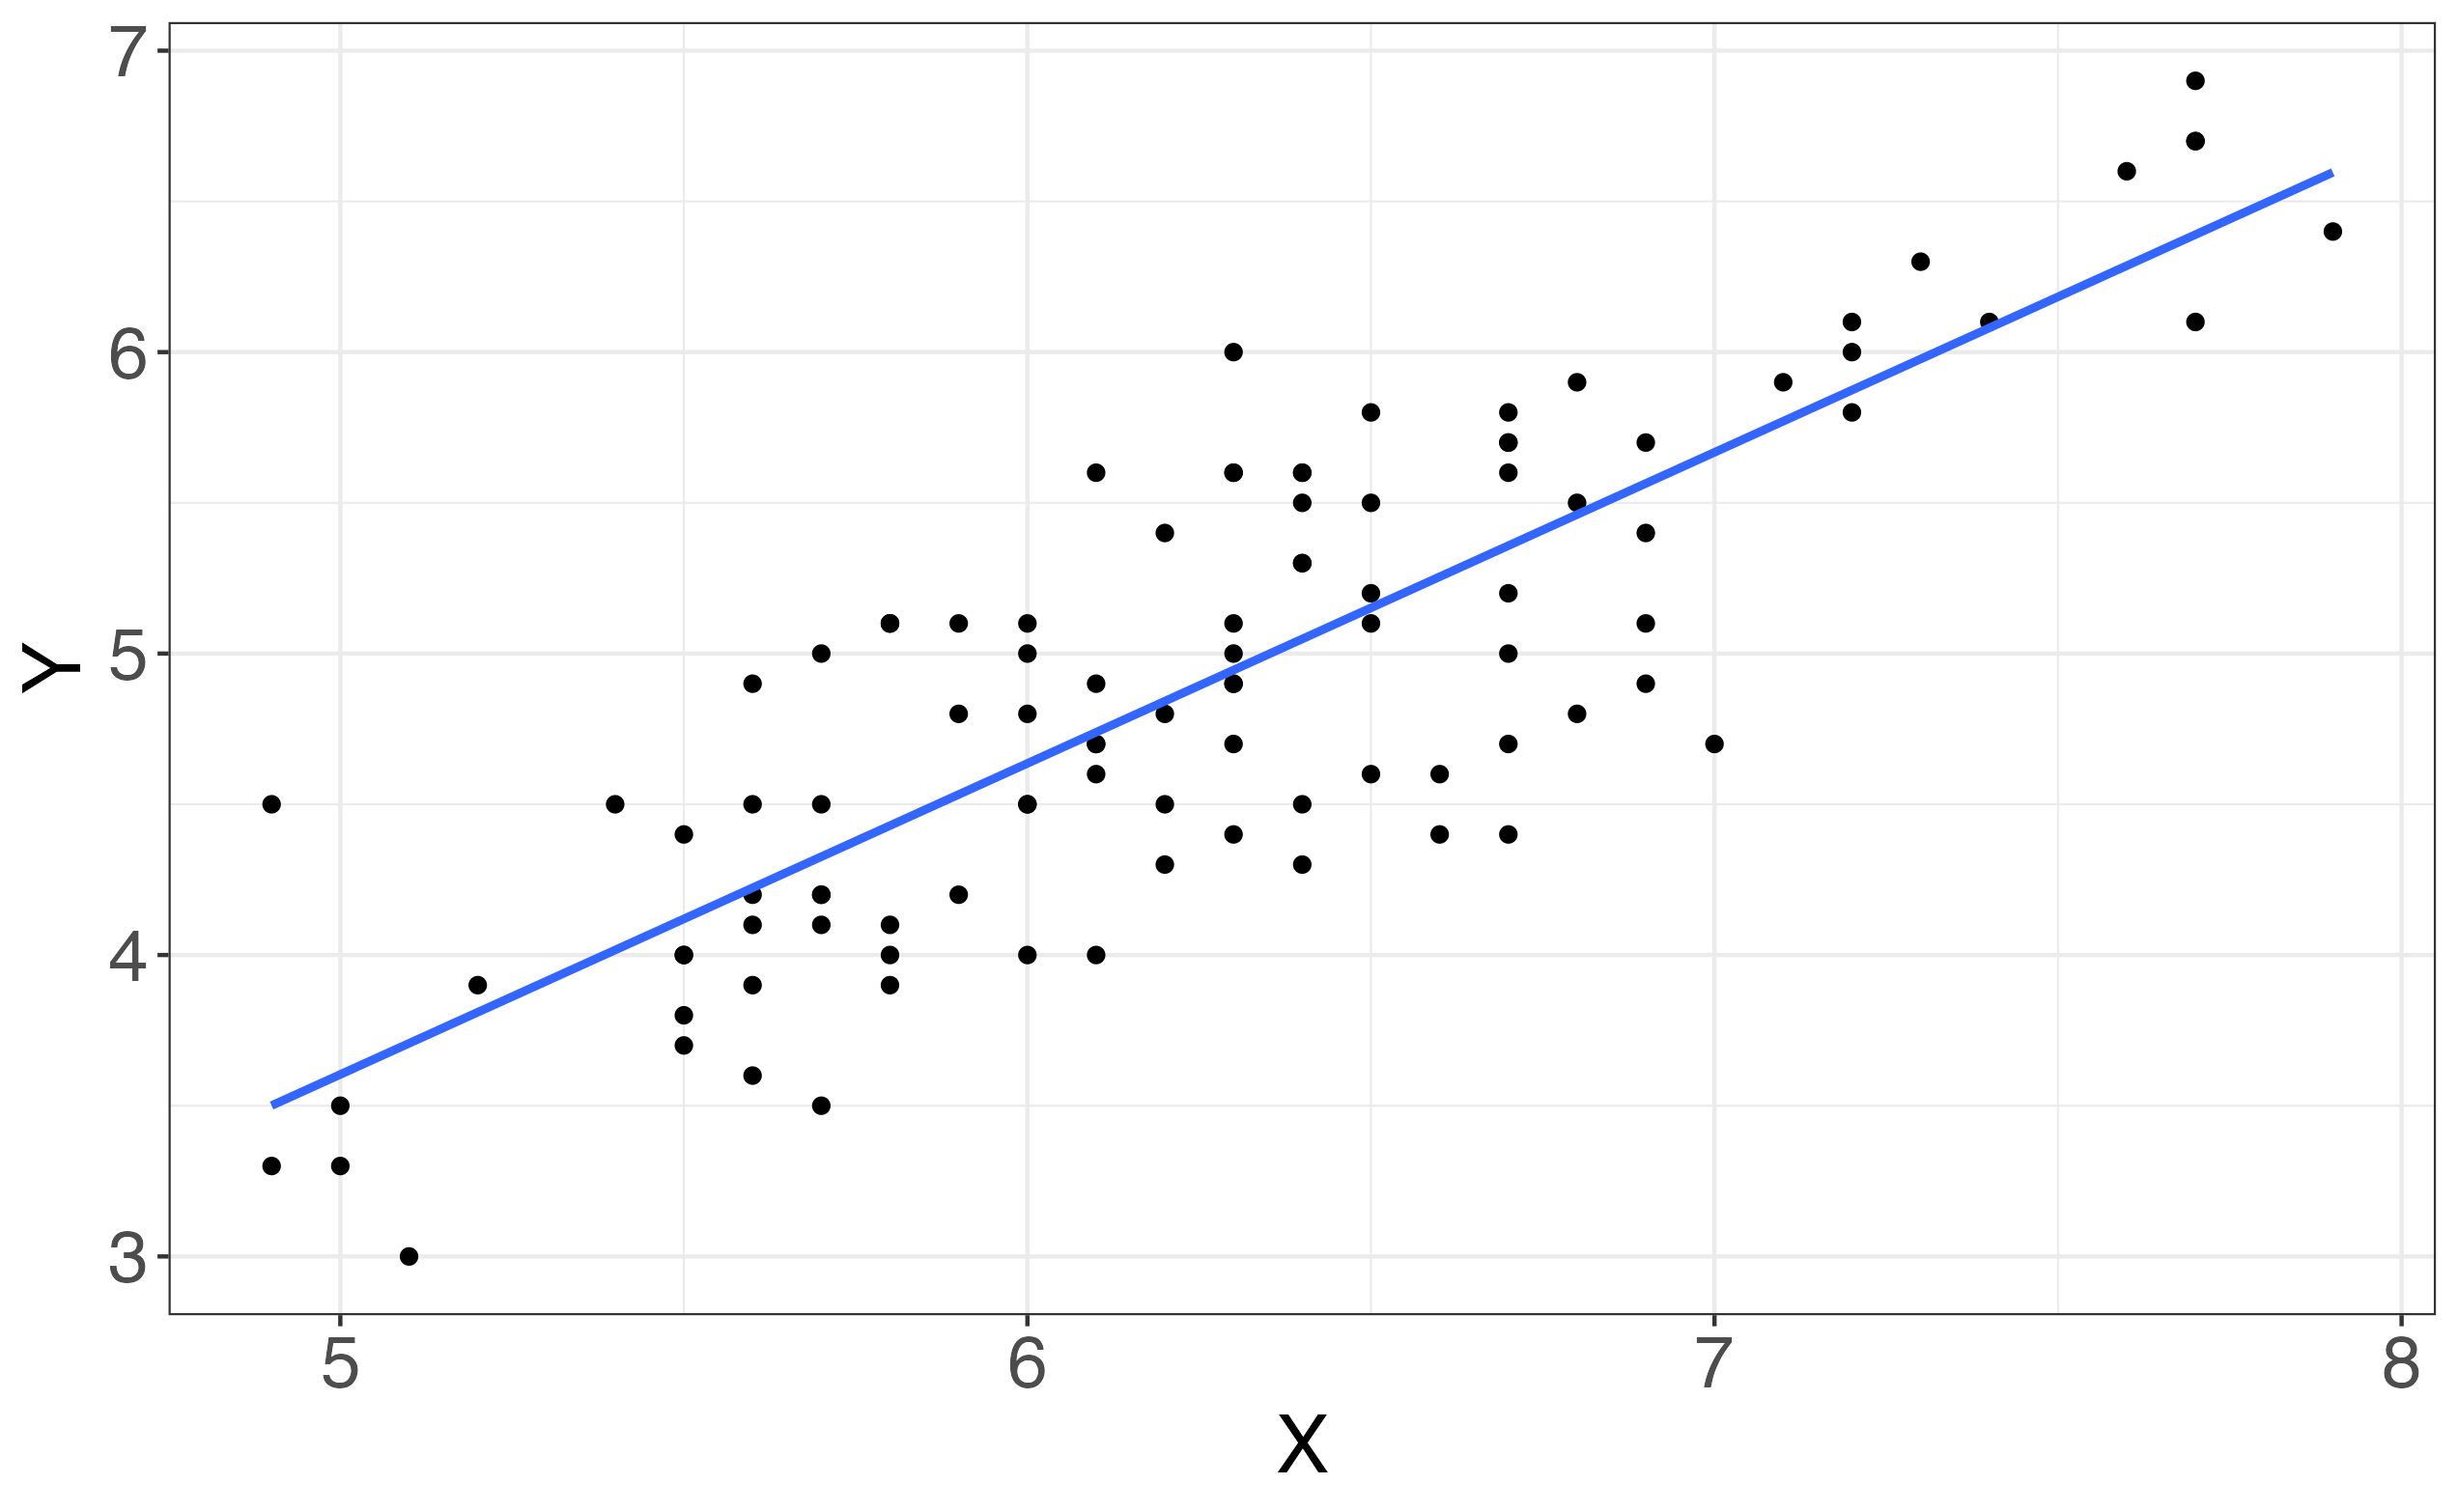
\includegraphics[scale=0.4]{figures/fitted_vals1.png}
%\end{frame}

\begin{frame}{Fitted values: Visualizing in two dimensions}
In two dimensions (where we have only one predictor $X_1$), we can visualize fitted values on a scatter plot:
\bigskip

\centering 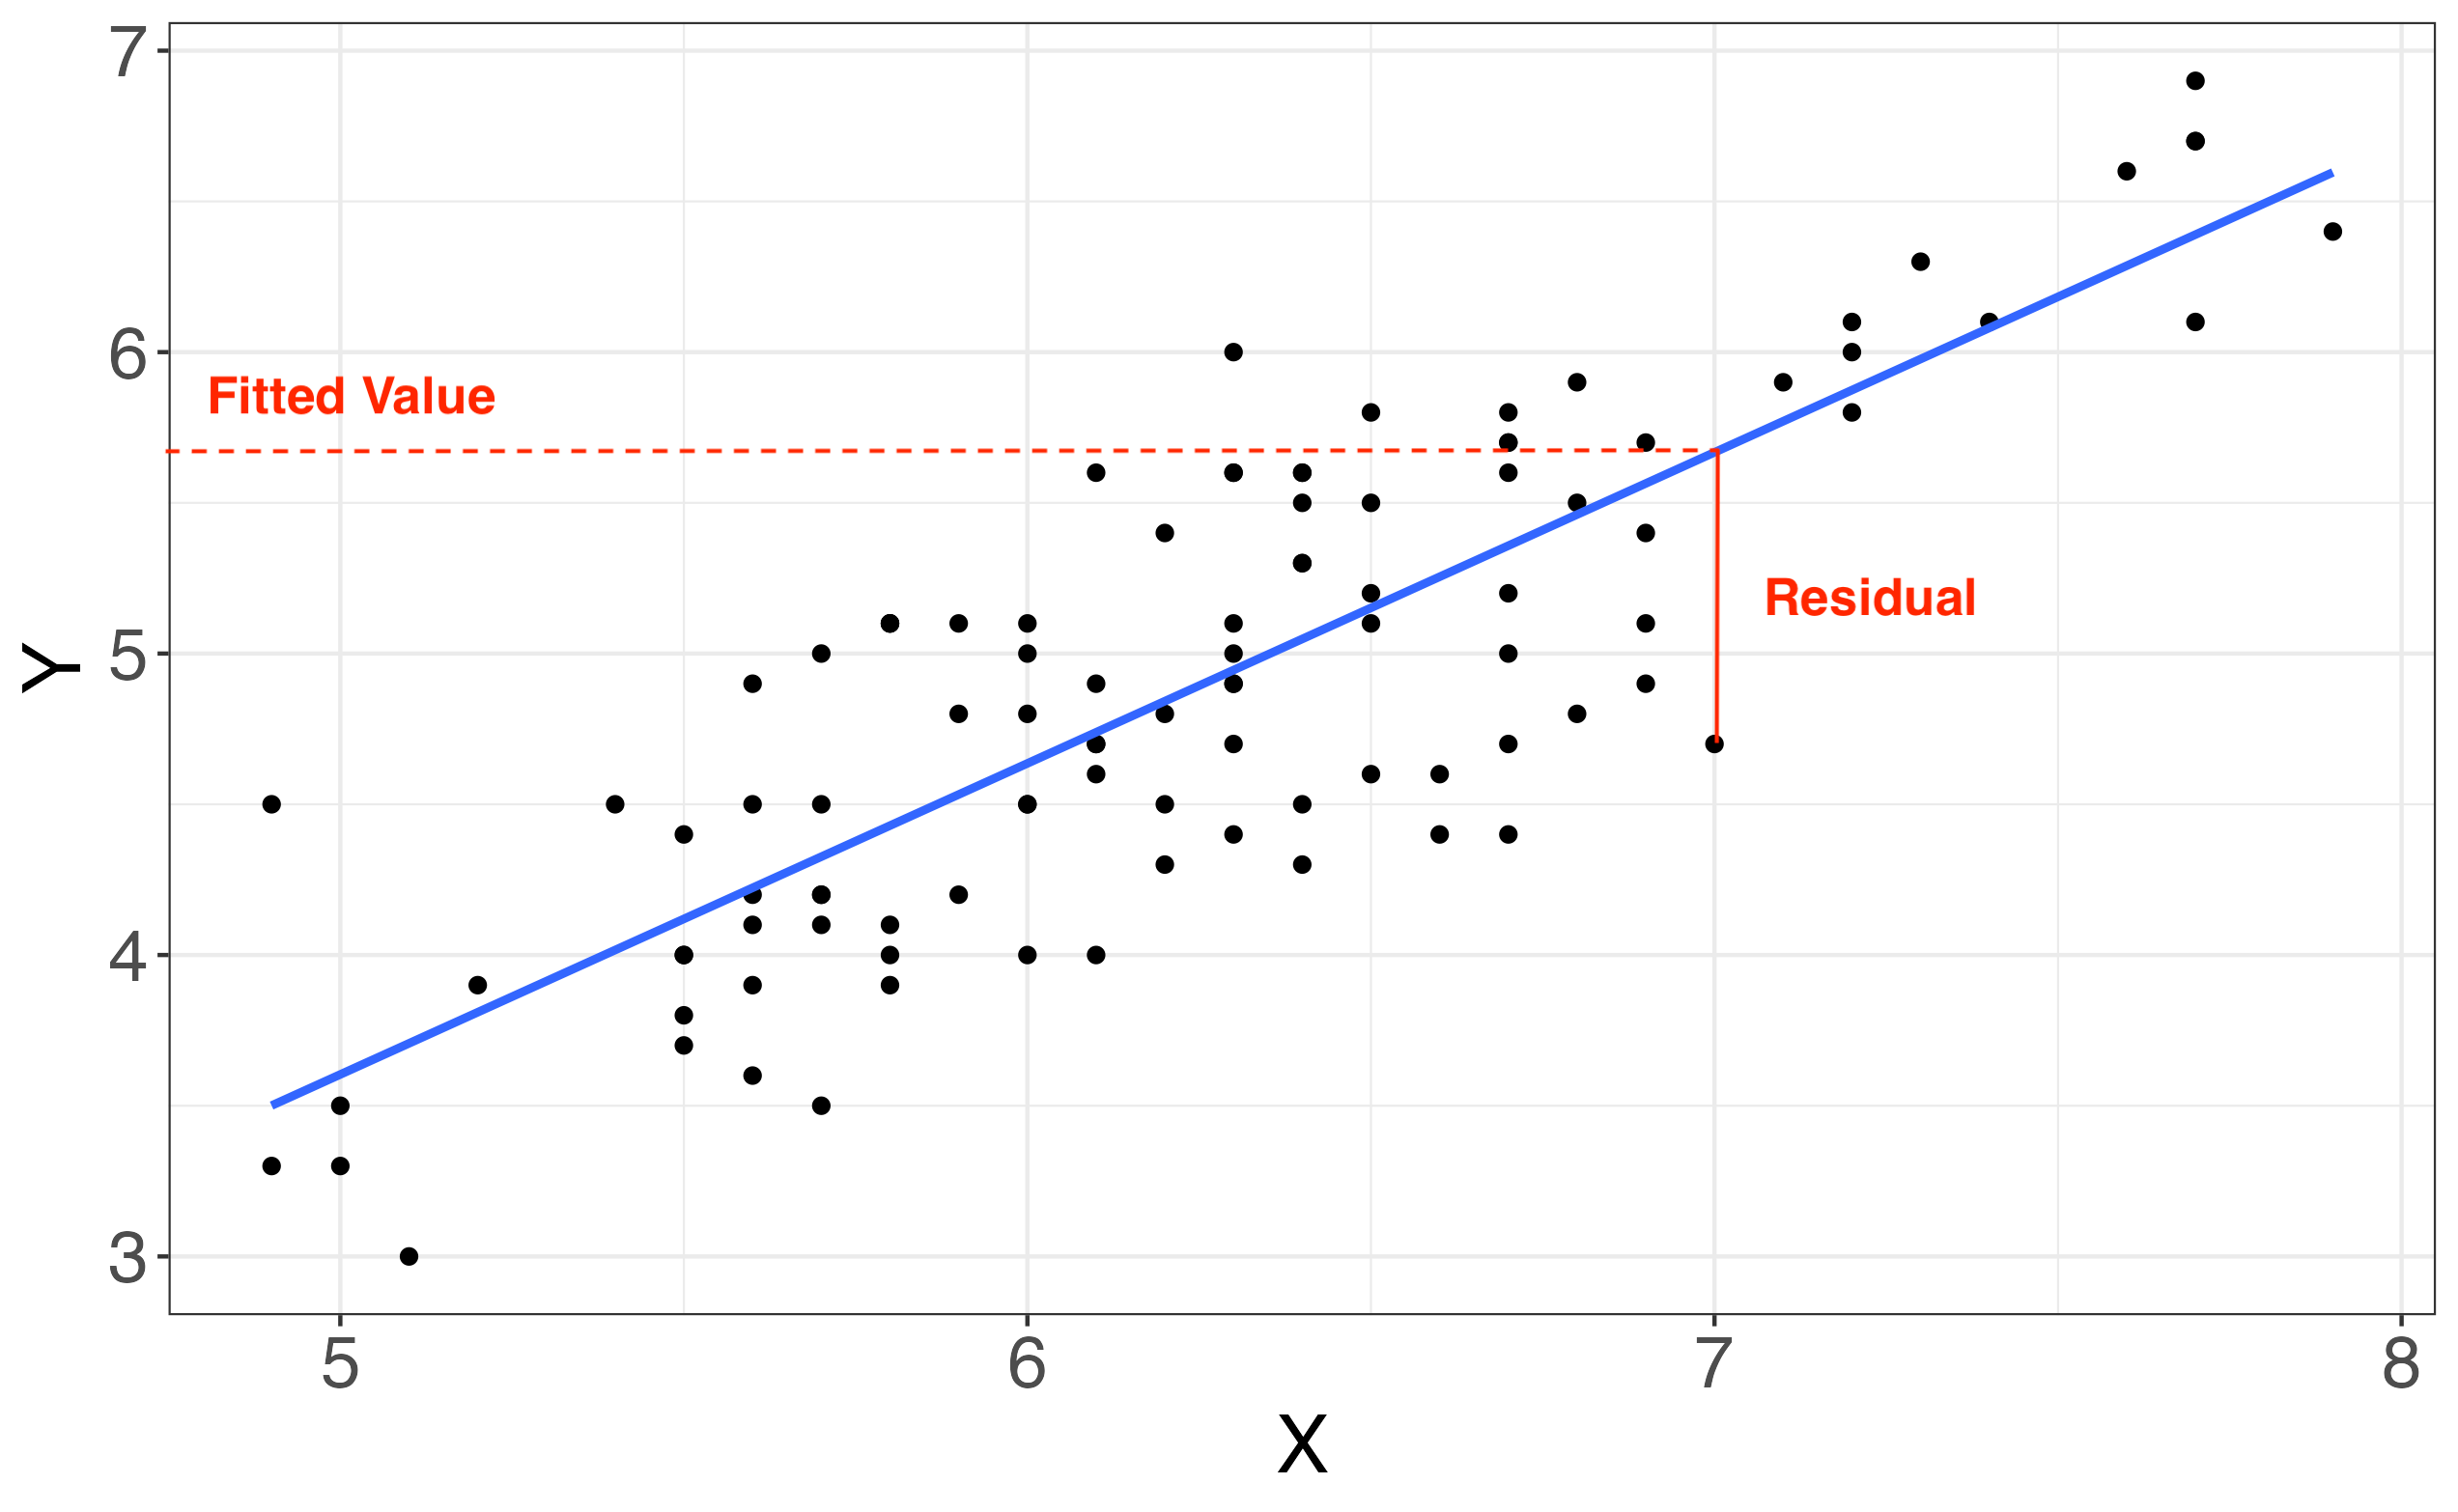
\includegraphics[scale=0.4]{figures/fitted_vals2.png}
\end{frame}

\begin{frame}{Fitted values and prediction}
Fitted values allow us to obtain predictions for each \textcolor{blue}{original} observation in our dataset.  

\vspace{0.3cm} 

\textcolor{blue}{Question:} How can we obtain a prediction for a \textcolor{blue}{new} observation based on its covariates? 

\vspace{0.3cm}

We can plug the covariates into our regression equation! We can denote this new observation as the $(n + 1)$'th observation, and write
$$
\hat{Y}_{n + 1} = \hat{\beta}_0 + \hat{\beta}_1 X_{(n + 1), 1} + \dots + \hat{\beta}_p X_{(n + 1), p}
$$
\medskip

We can calculate by $\hat{Y}_{n + 1}$ by hand or in \texttt{R}, and we'll see examples of both.

\end{frame}

\begin{frame}{Prediction: ``by hand"}
\vspace{-5 mm}

Suppose we're interested in predicting a baby's birthweight based on birth parent's age, marital status, whether or not they smoke during pregnancy, and weight prior to pregnancy. We can fit the appropriate regression model in \texttt{R}:

\vspace{0.2cm}

\centering 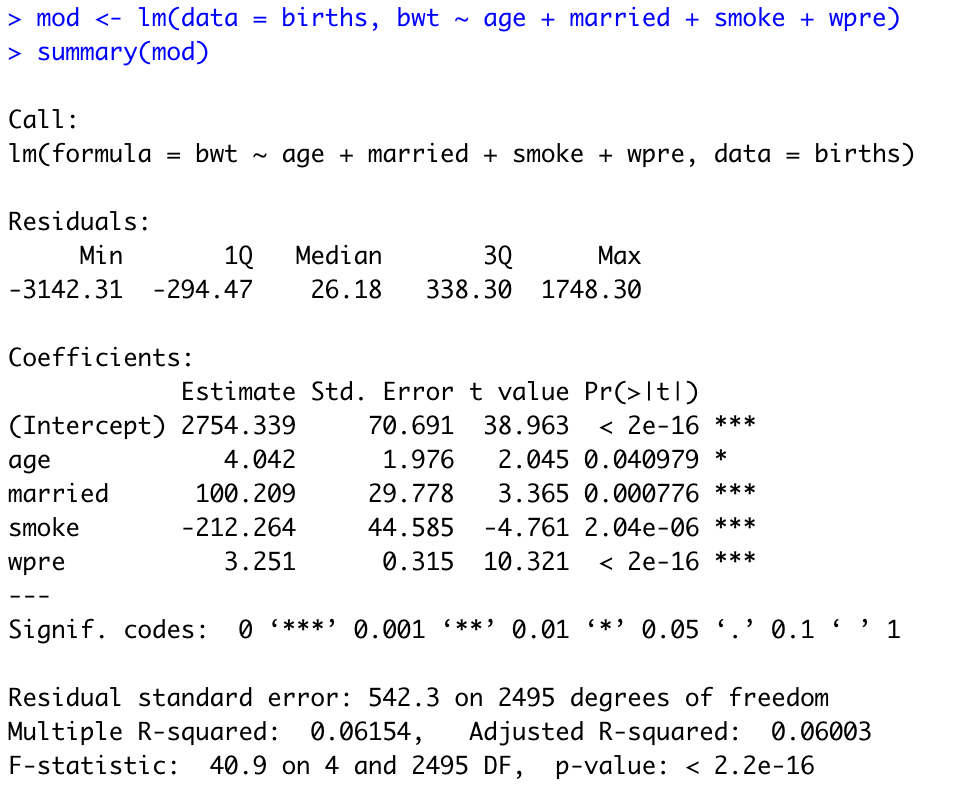
\includegraphics[scale=0.4]{figures/predict_reg.png}
\end{frame}

\begin{frame}{Prediction: ``by hand"}
Extracting the coefficient estimates from this model and plugging them into our regression equation, we get
\begin{align*}
\widehat{\texttt{bwt}} = & 2754.339 + 4.042 \times \texttt{age} + 100.209 \times \texttt{married} \\
& - 212.264 \times \texttt{smoke} + 3.251 \times \texttt{wpre} 
\end{align*} 

What is our best estimate of a baby's birthweight born to a birth parent who is \textcolor{blue}{25} years old, \textcolor{green}{married}, \textcolor{orange}{does not smoke}, and weighed \textcolor{violet}{150} pounds prior to pregnancy? 

\begin{align*}
\widehat{\texttt{bwt}} = & 2754.339 + 4.042 \times \textcolor{blue}{25} + 100.209 \times \textcolor{green}{1} \\
& - 212.264 \times \textcolor{orange}{0} + 3.251 \times \textcolor{violet}{150}  \\
& = 3443.223 \text{ grams}
\end{align*}

\end{frame}

\begin{frame}{Prediction: Example in \texttt{R}}
Extracting the coefficient estimates from this model and plugging them into our regression equation, we get
\begin{align*}
	\widehat{\texttt{bwt}} = & 2754.339 + 4.042 \times \texttt{age} + 100.209 \times \texttt{married} \\
	& - 212.264 \times \texttt{smoke} + 3.251 \times \texttt{wpre} 
\end{align*}

What is our best estimate of a baby's birthweight born to a birth parent who is \textcolor{blue}{20} years old, \textcolor{green}{umarried}, \textcolor{orange}{does smoke}, and weighed \textcolor{violet}{120} pounds prior to pregnancy?

\begin{align*}
\widehat{\texttt{bwt}} = & 2754.339 + 4.042 \times \textcolor{blue}{20} + 100.209 \times \textcolor{green}{0} \\
& - 212.264 \times \textcolor{orange}{1} + 3.251 \times \textcolor{violet}{120}  \\
& = 3443.223 \text{ grams}
\end{align*}

\end{frame}

\begin{frame}{Prediction: extrapolation}
Extracting the coefficient estimates from this model and plugging them into our regression equation, we get
\begin{align*}
	\widehat{\texttt{bwt}} = & 2754.339 + 4.042 \times \texttt{age} + 100.209 \times \texttt{married} \\
	& - 212.264 \times \texttt{smoke} + 3.251 \times \texttt{wpre} 
\end{align*}

What is our best estimate of a baby's birthweight born to a birth parent who is \textcolor{blue}{80} years old, \textcolor{green}{umarried}, \textcolor{orange}{does smoke}, and weighed \textcolor{violet}{1000} pounds prior to pregnancy?

\begin{align*}
\widehat{\texttt{bwt}} = & 2754.339 + 4.042 \times \textcolor{blue}{80} + 100.209 \times \textcolor{green}{0} \\
& - 212.264 \times \textcolor{orange}{1} + 3.251 \times \textcolor{violet}{1000}  \\
& = 3443.223 \text{ grams}
\end{align*}

* 6428.78 grams is approximately 13.3 pounds

\end{frame}


\begin{frame}{Prediction: extrapolation}
	\vspace{-0.5cm}
Our birthweight estimate for a birth parent who is 80 years old, unmarried, does smoke, and weighed 1000 pounds prior to pregnancy was 13.3 pounds. 13.3 pounds is not unheard of, but is very large.

\vspace{0.3cm}

\textcolor{blue}{Question:} Within our dataset, the oldest observed individual was 46 years old, and the individual with the highest pre-pregnancy birthweight was 350 pounds. Is it reasonable to make a prediction using covariate values so far outside of our observed range?  

\vspace{0.3cm}

\textcolor{blue}{Answer:} 
\begin{itemize}
\item If we believe that the observed linear relationship holds for covariate values even outside the range observed in our data, then we may be okay

\medskip

\item But we can't know if the linear relationship holds for covariate values outside of the data range, because we don't observe them! 

\medskip

\item Predicting values outside of the range of our observed data is \textcolor{blue}{extrapolation}, and is unreasonable in many scientific settings.
\end{itemize}
\end{frame}

\begin{frame}{Prediction: using \texttt{R}}
Rather than calculate predictions by hand, it is often useful to do this in \texttt{R}, and we can make predictions for more than one observation at a time.

\vspace{0.3cm}

To get fitted values for our \textcolor{blue}{observed} data, we call the \texttt{predict} function on our modeling object \texttt{mod} (where \texttt{mod} is the output of a regression model):

\vspace{0.3cm}

\texttt{fitted\_vals <- predict(mod)}


\bigskip

\textcolor{blue}{Question}: We have already used this code. What do we use it for?

\end{frame}


\begin{frame}{Prediction: using \texttt{R}}
To get fitted values for \textcolor{blue}{new} data, we use the \texttt{newdata} argument inside of \texttt{predict}:

\vspace{0.3cm}

\texttt{new\_df <- data.frame(...)} \\
\texttt{fitted\_vals <- predict(mod, newdata = new\_df)}

\vspace{0.3cm}

where \texttt{new\_df} is a dataframe that contains columns for all covariates in your model.

\end{frame}

\begin{frame}{Prediction: using \texttt{R}}
Earlier we calculated by hand our best estimate of a baby's birthweight born to a birth parent who is 25 years old, married, does not smoke, and weighed 150 pounds prior to pregnancy. In \texttt{R}, we can use the following code:

\vspace{0.3cm}

\begin{figure}
	\centering 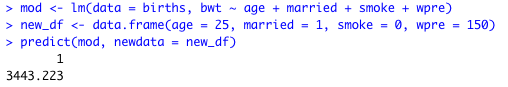
\includegraphics[scale=0.5]{figures/newdata_example.png}
\end{figure}

\vspace{0.3cm}

\texttt{new\_df} is a dataframe containing a single row (one observation), for someone who is 25 years old, married, does not smoke, and weighed 150 pounds prior to pregnancy. \texttt{R} does all of the math for us!

\end{frame}

\begin{frame}{Prediction: Example in \texttt{R}}
We can also make predictions for multiple observations at the same time. For example, we can make predictions for all three of our examples from earlier using just a few lines of code:

\bigskip

\centering 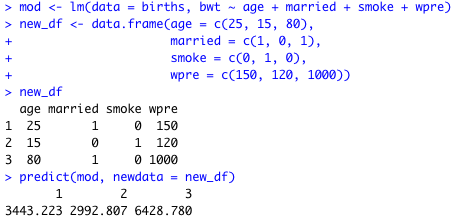
\includegraphics[scale=0.6]{figures/newdata_example2.png}

\end{frame}
\vspace{-10 mm}
% could include a slide about thinking about which variables you can include in your model (i.e. not sex of child if we're predicting birthweight because not everyone knows the sex of their child before birth)
\begin{frame}{\textcolor{violet}{Pollev:} Example in \texttt{R}}
	What is the predicted birth weight in grams for a baby born to a parent who is age 15, is not married, does smoke, and weighed 120 pounds before pregnancy? (rounding to the nearest gram)\\
	\tiny{\url{https://PollEv.com/multiple_choice_polls/D8xSCL4m5LICgVmDadTGa/respond}}
	
	\medskip
	
	\begin{figure}
	\centering 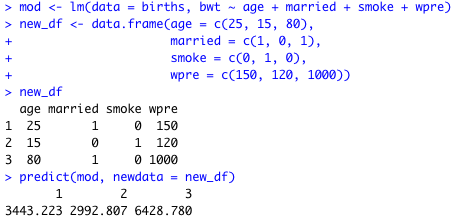
\includegraphics[scale=0.6]{figures/newdata_example2.png}
\end{figure}\pause
\normalsize
 \textcolor{blue}{about 2993 grams}
	
\end{frame}

\begin{frame}
	Question: What could be an issue with including a variable like weight of the baby at one month in this model?
	\bigskip
	
	What could be an issue with including a variable like sex of the baby in this model?
	
\end{frame}





\section{Measures of prediction accuracy}

\begin{frame}
 We now know how to predict the outcomes of observed and new data using a linear regression model.
 
 \bigskip
 
 But how do we choose the model in the first place?
 
 \bigskip
 
 In order to choose a model, we need to be able to \textcolor{blue}{evaluate} how \textcolor{blue}{accurate} our models are.
 
 \bigskip
 
 We will look at two measure of prediction accuracy for continuous outcomes:
 \medskip
 \begin{itemize}
 	\item $R^2$
 	\smallskip
 	\item Mean Squared Error (MSE)
 \end{itemize}
 
\end{frame}

\subsection{$R^2$}


\begin{frame}{$R^2$: Coefficient of determination}

\vspace{-5 mm}

\textcolor{blue}{$R^2$ (also called the coefficient of determination)}: 
\medskip
\begin{itemize}
\item the proportion of the variance in the outcome explained by the covariates in the model. 
\medskip
\item for simple linear regression, $R^2$ is the square of the correlation
\medskip

\item  often used for \textcolor{blue}{model comparison}, where we have a set of possible predictive models and are trying to determine which is best.
\end{itemize}

\vspace{0.3cm}

\textcolor{blue}{$R^2$ can take values between 0 and 1}:

\vspace{0.3cm}

\begin{itemize}
	\item If $R^2$ is close to 0, then the covariates in our predictive model don't do a good job of explaining the variation in the outcome
	
	\medskip
	
	\item If $R^2$ is close to 1, then the covariates in our predictive model do a good job of explaining the variation in the outcome
\end{itemize}


\end{frame}

\begin{frame}{$R^2$: Multiple vs. Adjusted}
$R^2$ can be found in regression output from the \texttt{lm} function. The output gives us two types of $R^2$:

\vspace{0.3cm}

\begin{itemize}
	\item \textcolor{blue}{Multiple $R^2$}: $$1 - \frac{\sum_{i = 1}^n (Y_i - \hat{Y}_i)^2}{\sum_{i = 1}^n (Y_i - \bar{Y})^2} \hspace{0.3cm} 
\includegraphics[scale=0.01]{figures/technical.png}$$  [1 - (sum of squared residuals / total sum of squares)] 
	
	\bigskip
	
	\item \textcolor{blue}{Adjusted $R^2$}: Similar to $R^2$, but accounts for the number of covariates in the model
\end{itemize}

\end{frame}

\begin{frame}{$R^2$: Multiple vs. Adjusted}
Key information:

\vspace{0.3cm}

\begin{itemize}
	\item Multiple $R^2$ will  \textcolor{blue}{always} increase from adding additional covariates into a model
	\bigskip
	
	
	\item Adjusted $R^2$ will \textcolor{blue}{not always} increase from adding additional covariates into a model, because it \textcolor{blue}{penalizes adding additional variables}
	\bigskip
	
	\item Adjusted $R^2$ has a more complicated interpretation than $R^2$ 
\end{itemize}

\end{frame}

\begin{frame}{$R^2$: Multiple vs. Adjusted}

\textcolor{blue}{Question:} Suppose we are choosing between two predictive models. A higher $R^2$ means a higher proportion of variation in the outcome is being explained by the covariates in the model, so we're inclined to choose the model with higher $R^2$. \textcolor{blue}{Why might we prefer adjusted $R^2$ to multiple $R^2$? }

\bigskip

\textcolor{blue}{Answer:} Since multiple $R^2$ increases from adding additional covariates into a model, we would always be inclined to choose the model with the most covariates. This could lead us to choose a model that is \textcolor{orange}{overfit} to our data.

\end{frame}

\begin{frame}{Overfitting}

\textcolor{blue}{Overfitting}: when we fit a statistical model that corresponds too exactly to our observed data, which tends to lead to \textcolor{red}{worse predictions for new observations}.

\vspace{0.3cm}

Overfitting can involve:

\vspace{0.3cm}

\begin{itemize}
	\item Including too many covariates in a model 
	
	\medskip
	
	\item Making the relationship between the outcome and the given covariates too complicated
	\medskip
	
	\begin{itemize}
		\item An example of this is interpolation, where we fit a curve that must go through each data point
	\end{itemize}
\end{itemize}

\end{frame}

\begin{frame}{Overfitting: Example}
Suppose we collect data for an outcome $Y$ and predictor $X$. We visualize our data in the scatter plot below:

\vspace{0.3cm}

\centering 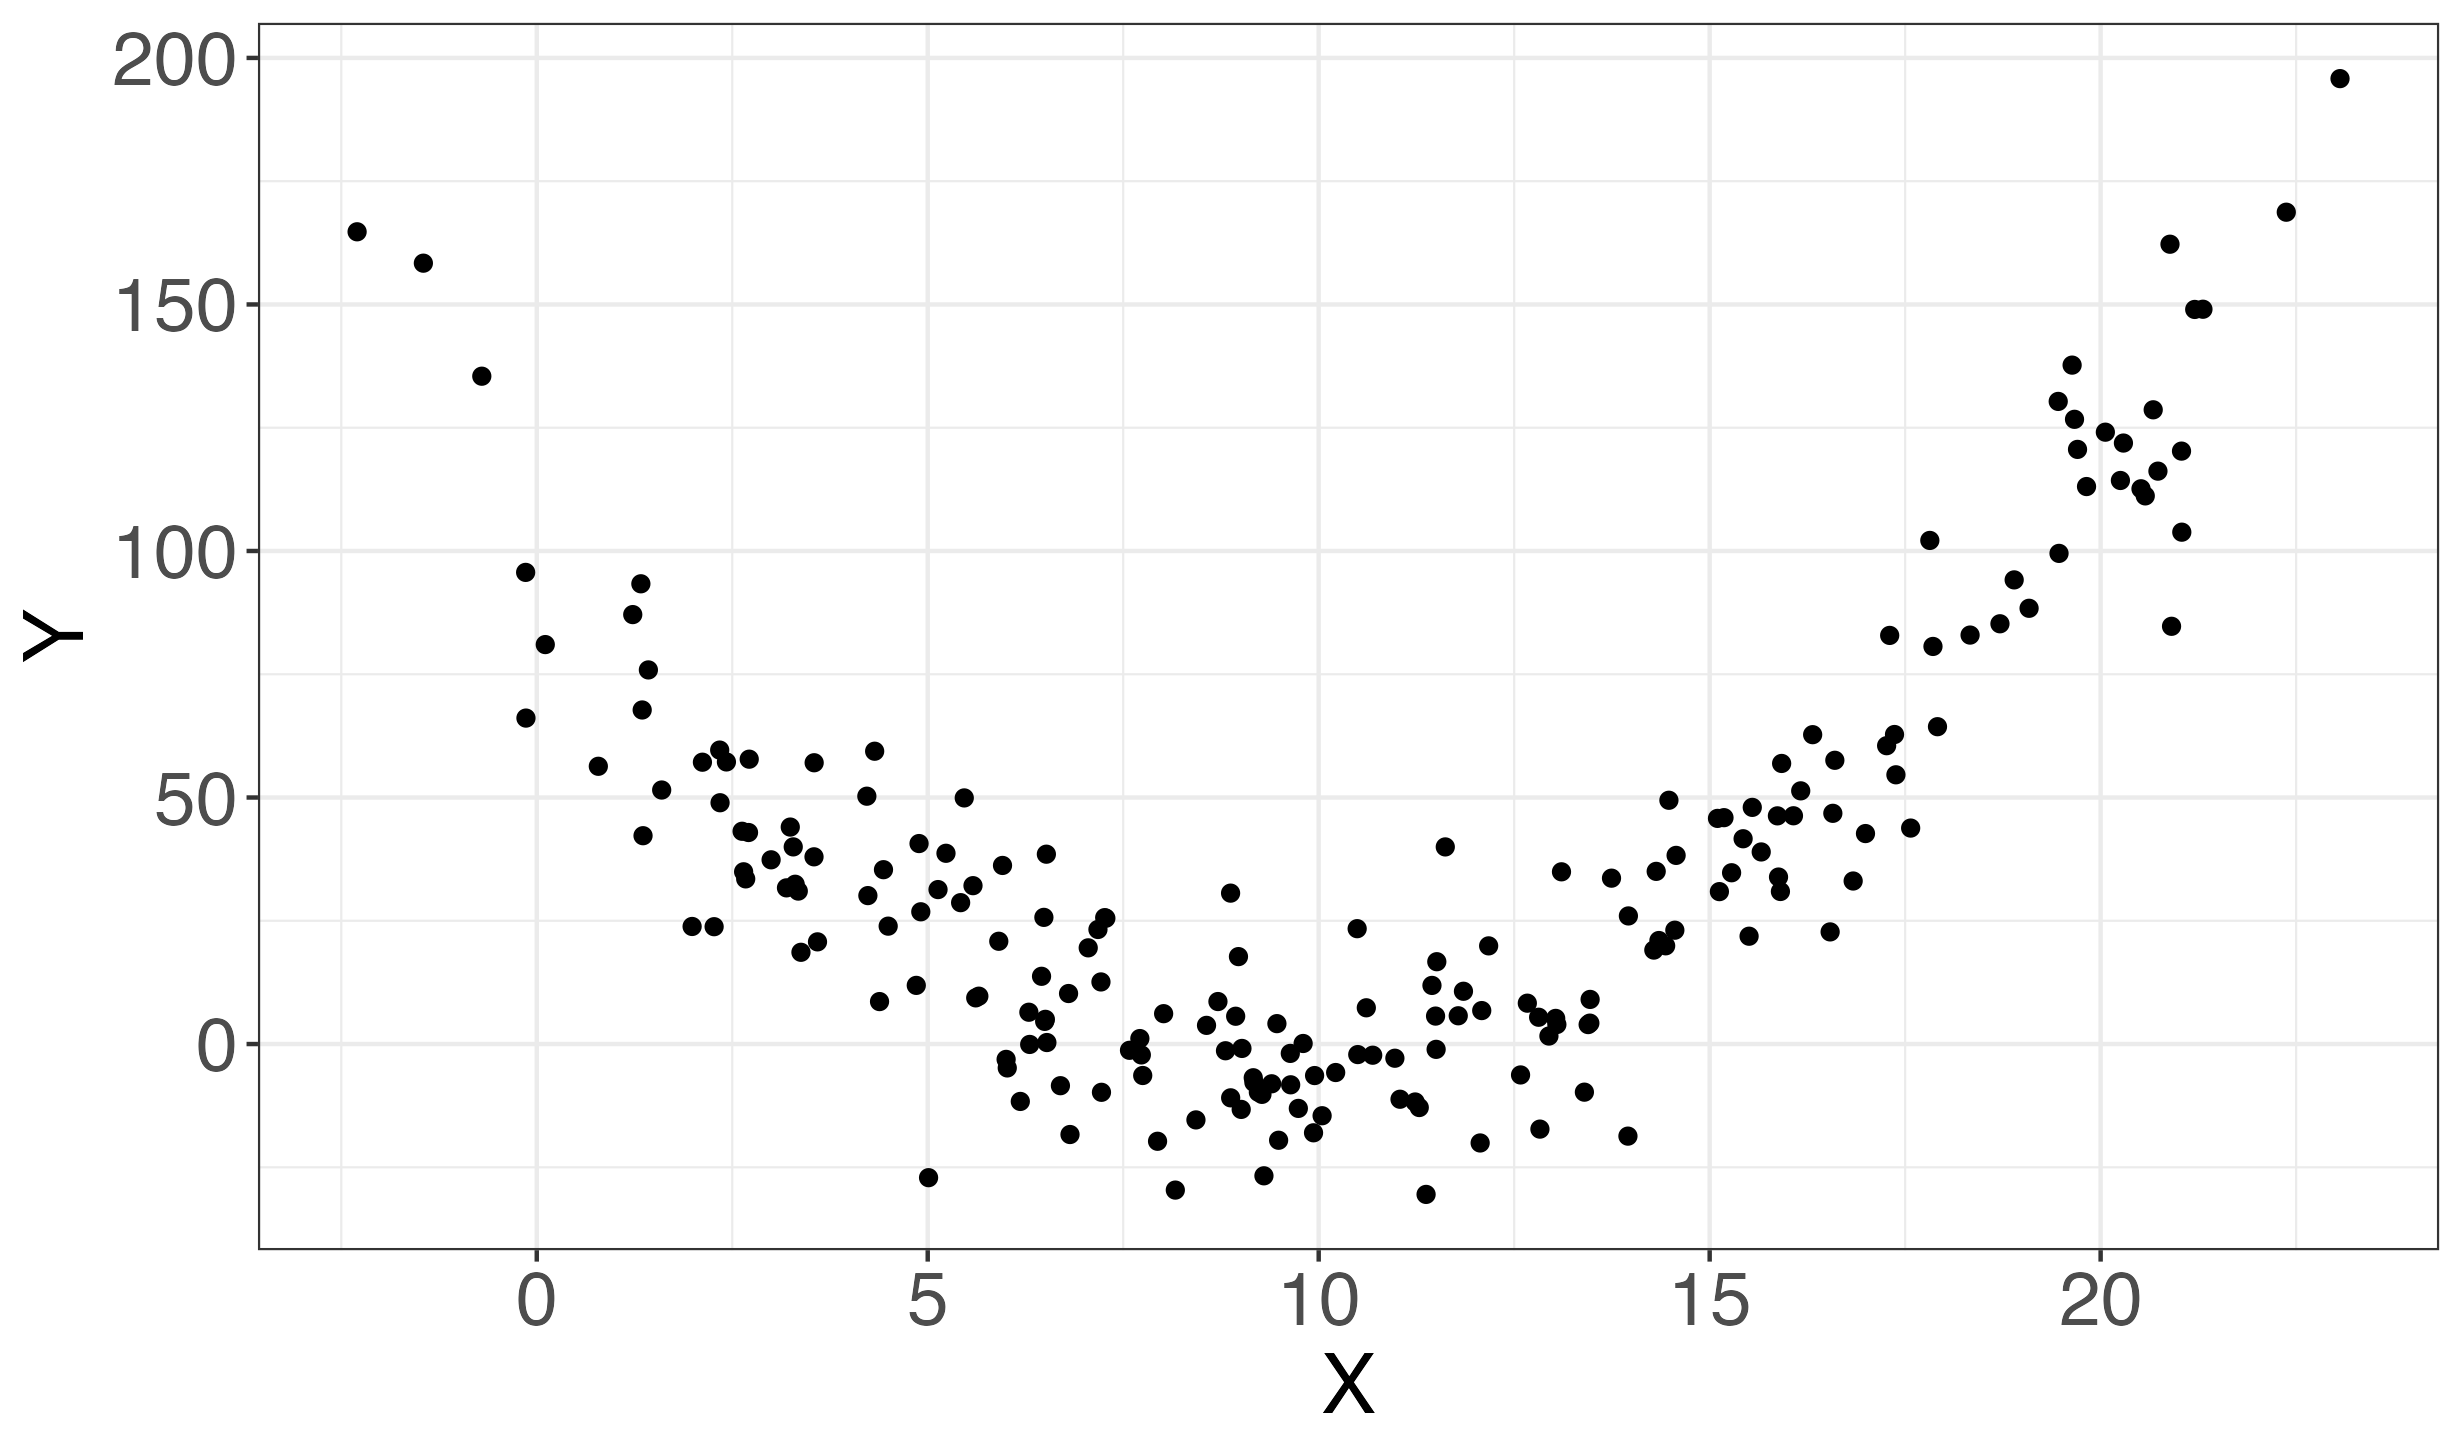
\includegraphics[scale=0.4]{figures/overfit1.png}
\end{frame}

\begin{frame}{Overfitting: Example}
We could fit a simple linear regression model to our data, but this likely wouldn't produce great predictions\dots

\vspace{0.3cm}

\centering 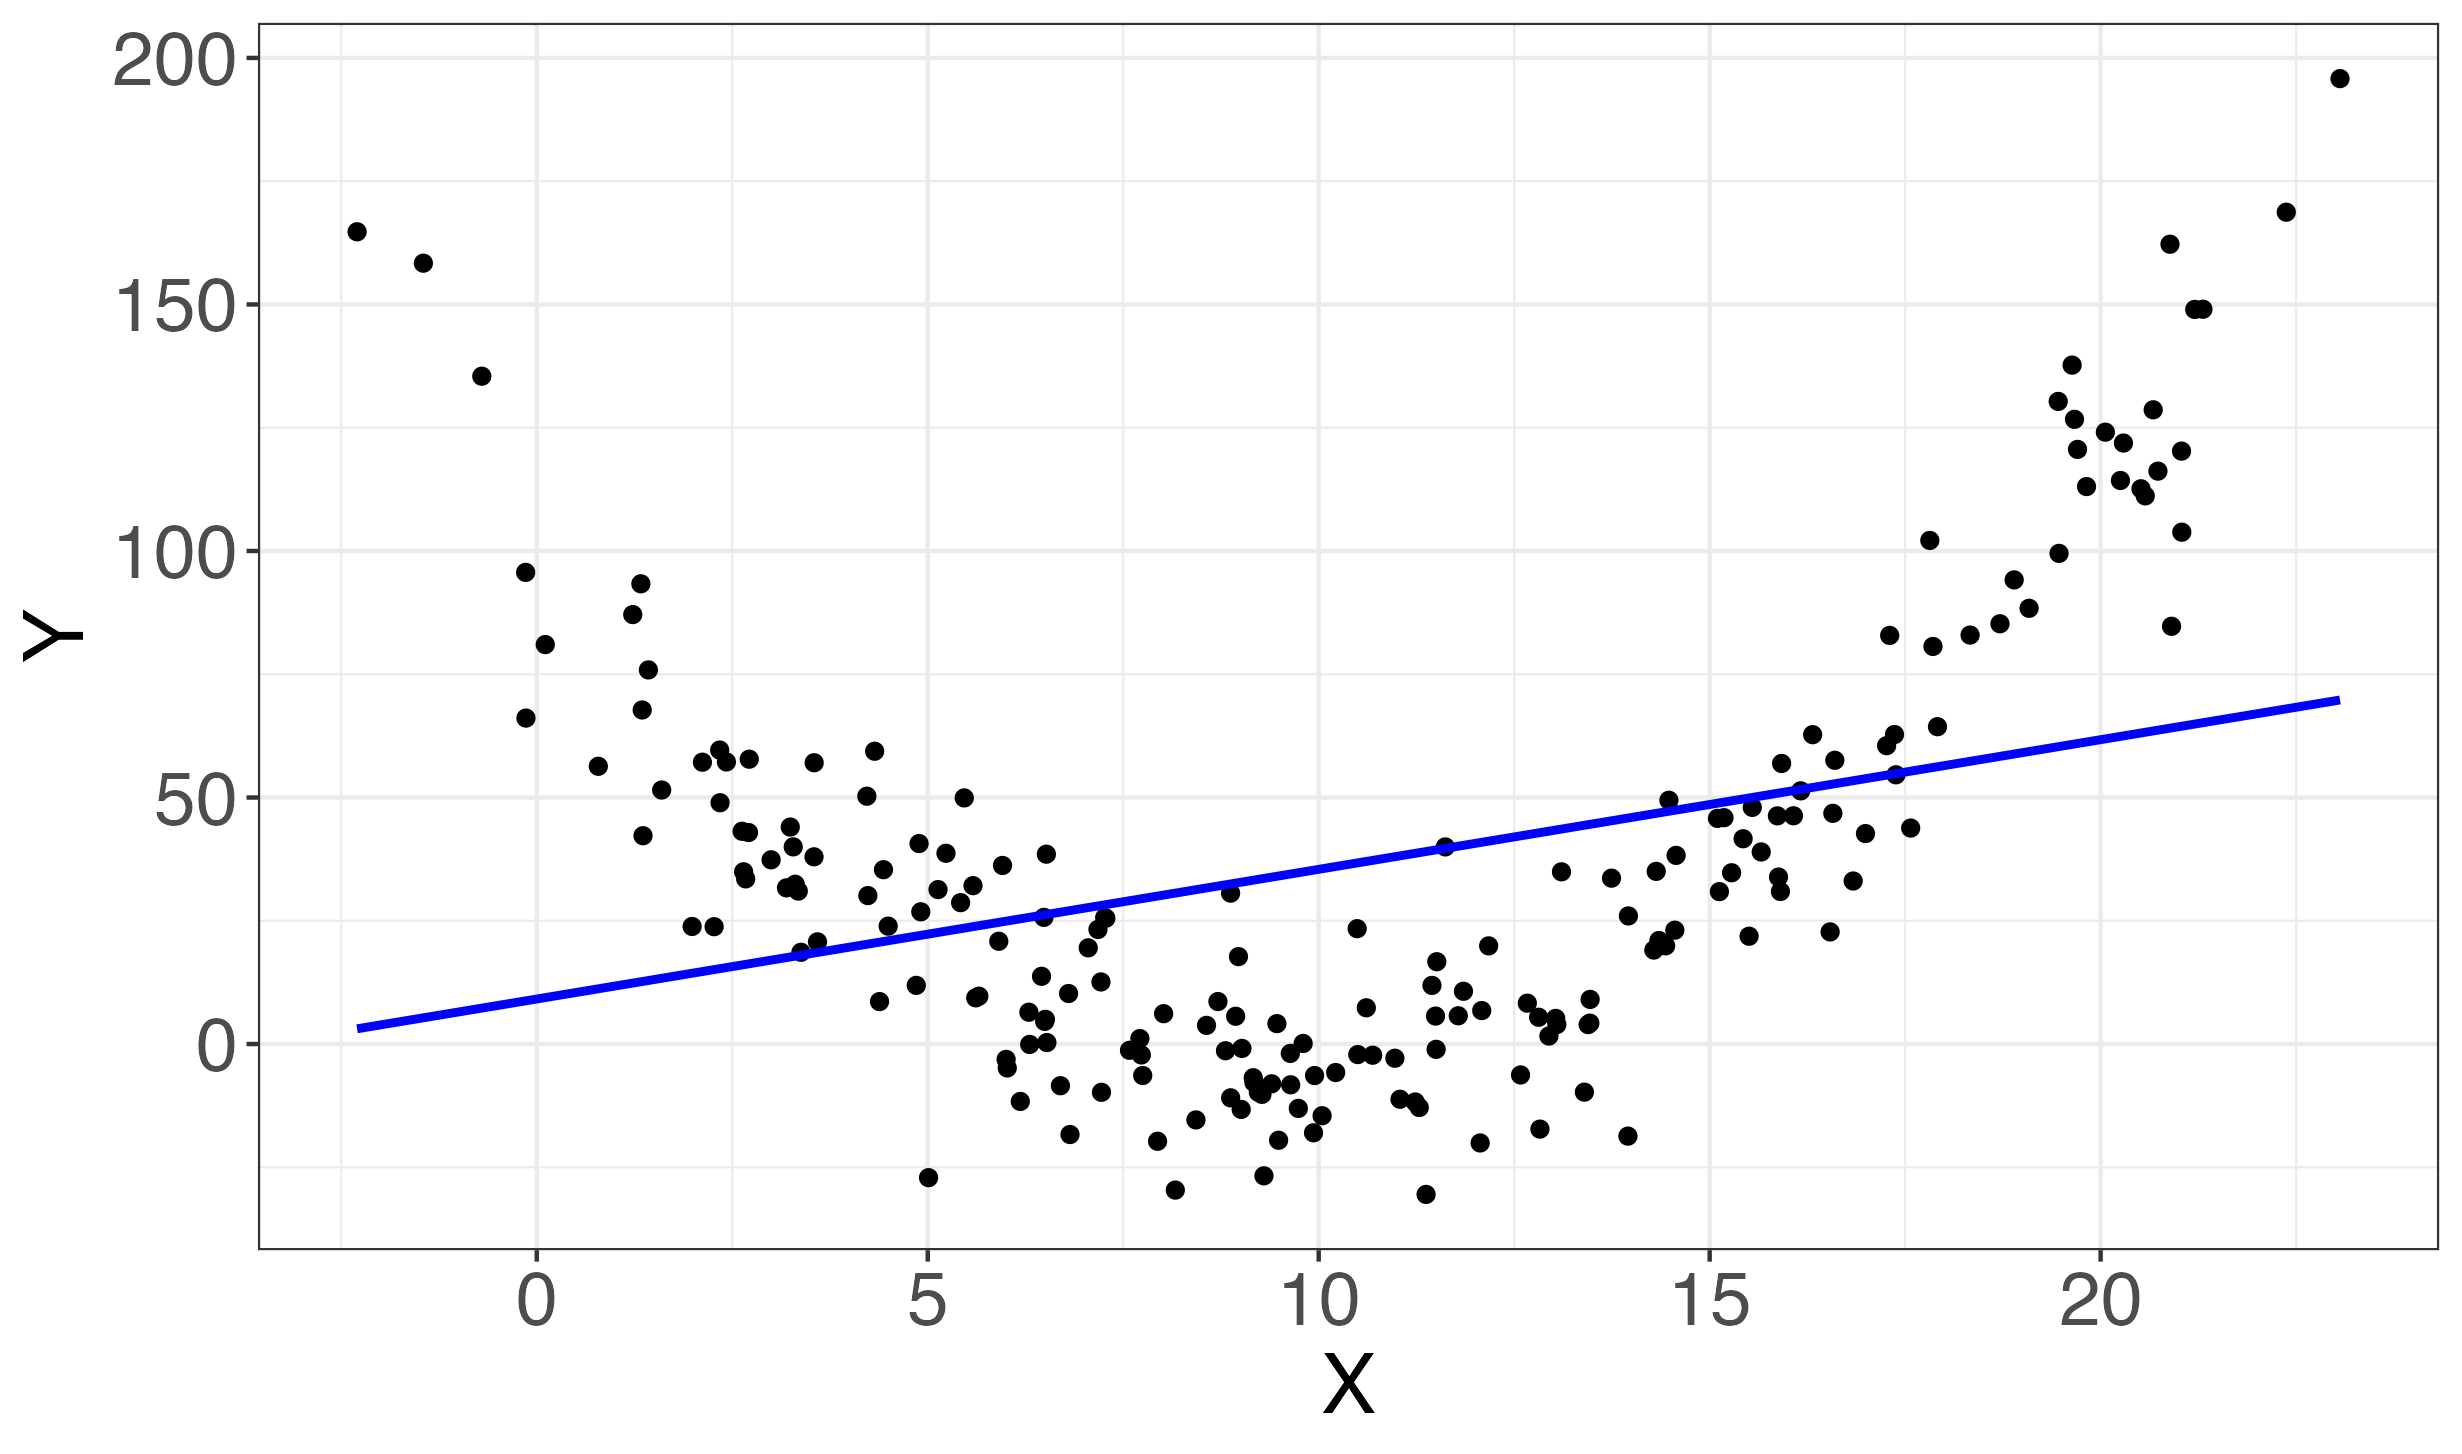
\includegraphics[scale=0.4]{figures/overfit2.png}
\end{frame}

\begin{frame}{Overfitting: Example}
We could add an additional covariate term to our model, namely $X^2$\dots

\vspace{0.3cm}

\centering 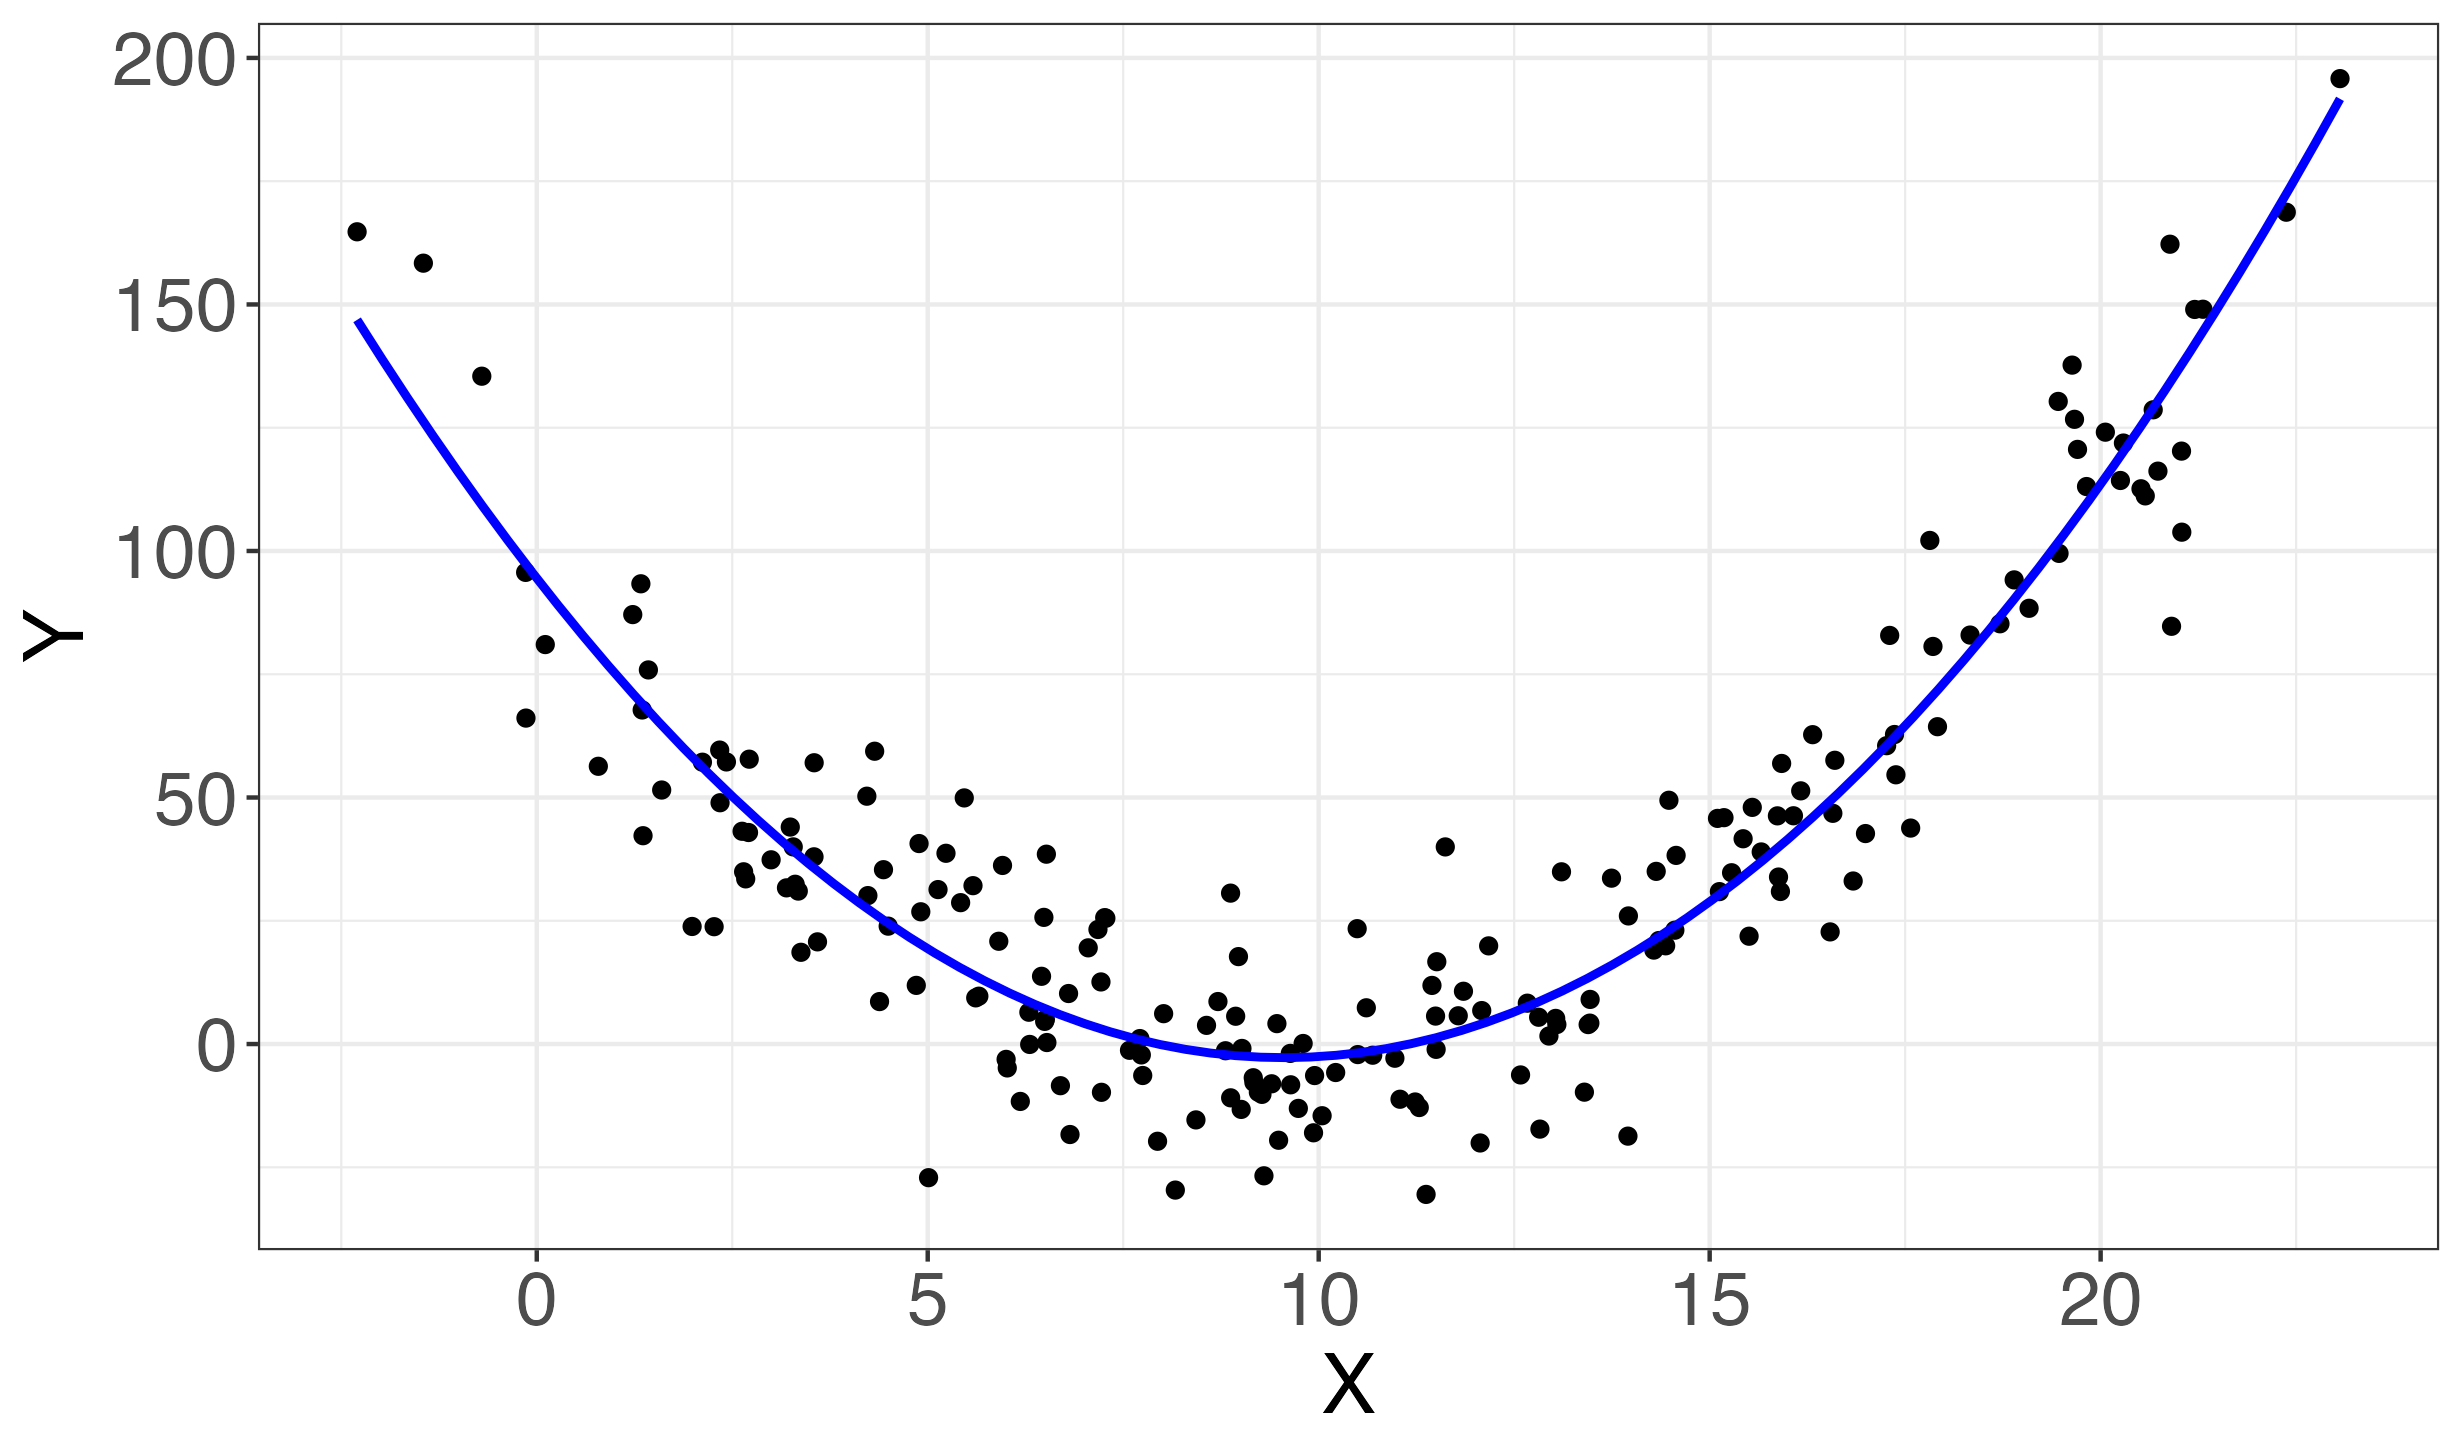
\includegraphics[scale=0.4]{figures/overfit3.png}

\end{frame}

\begin{frame}{Overfitting: Example}
Or we could include  \textcolor{blue}{many} additional covariate terms, for higher order polynomials (here, up to $X^{13}$)\dots

\vspace{0.3cm}

\centering 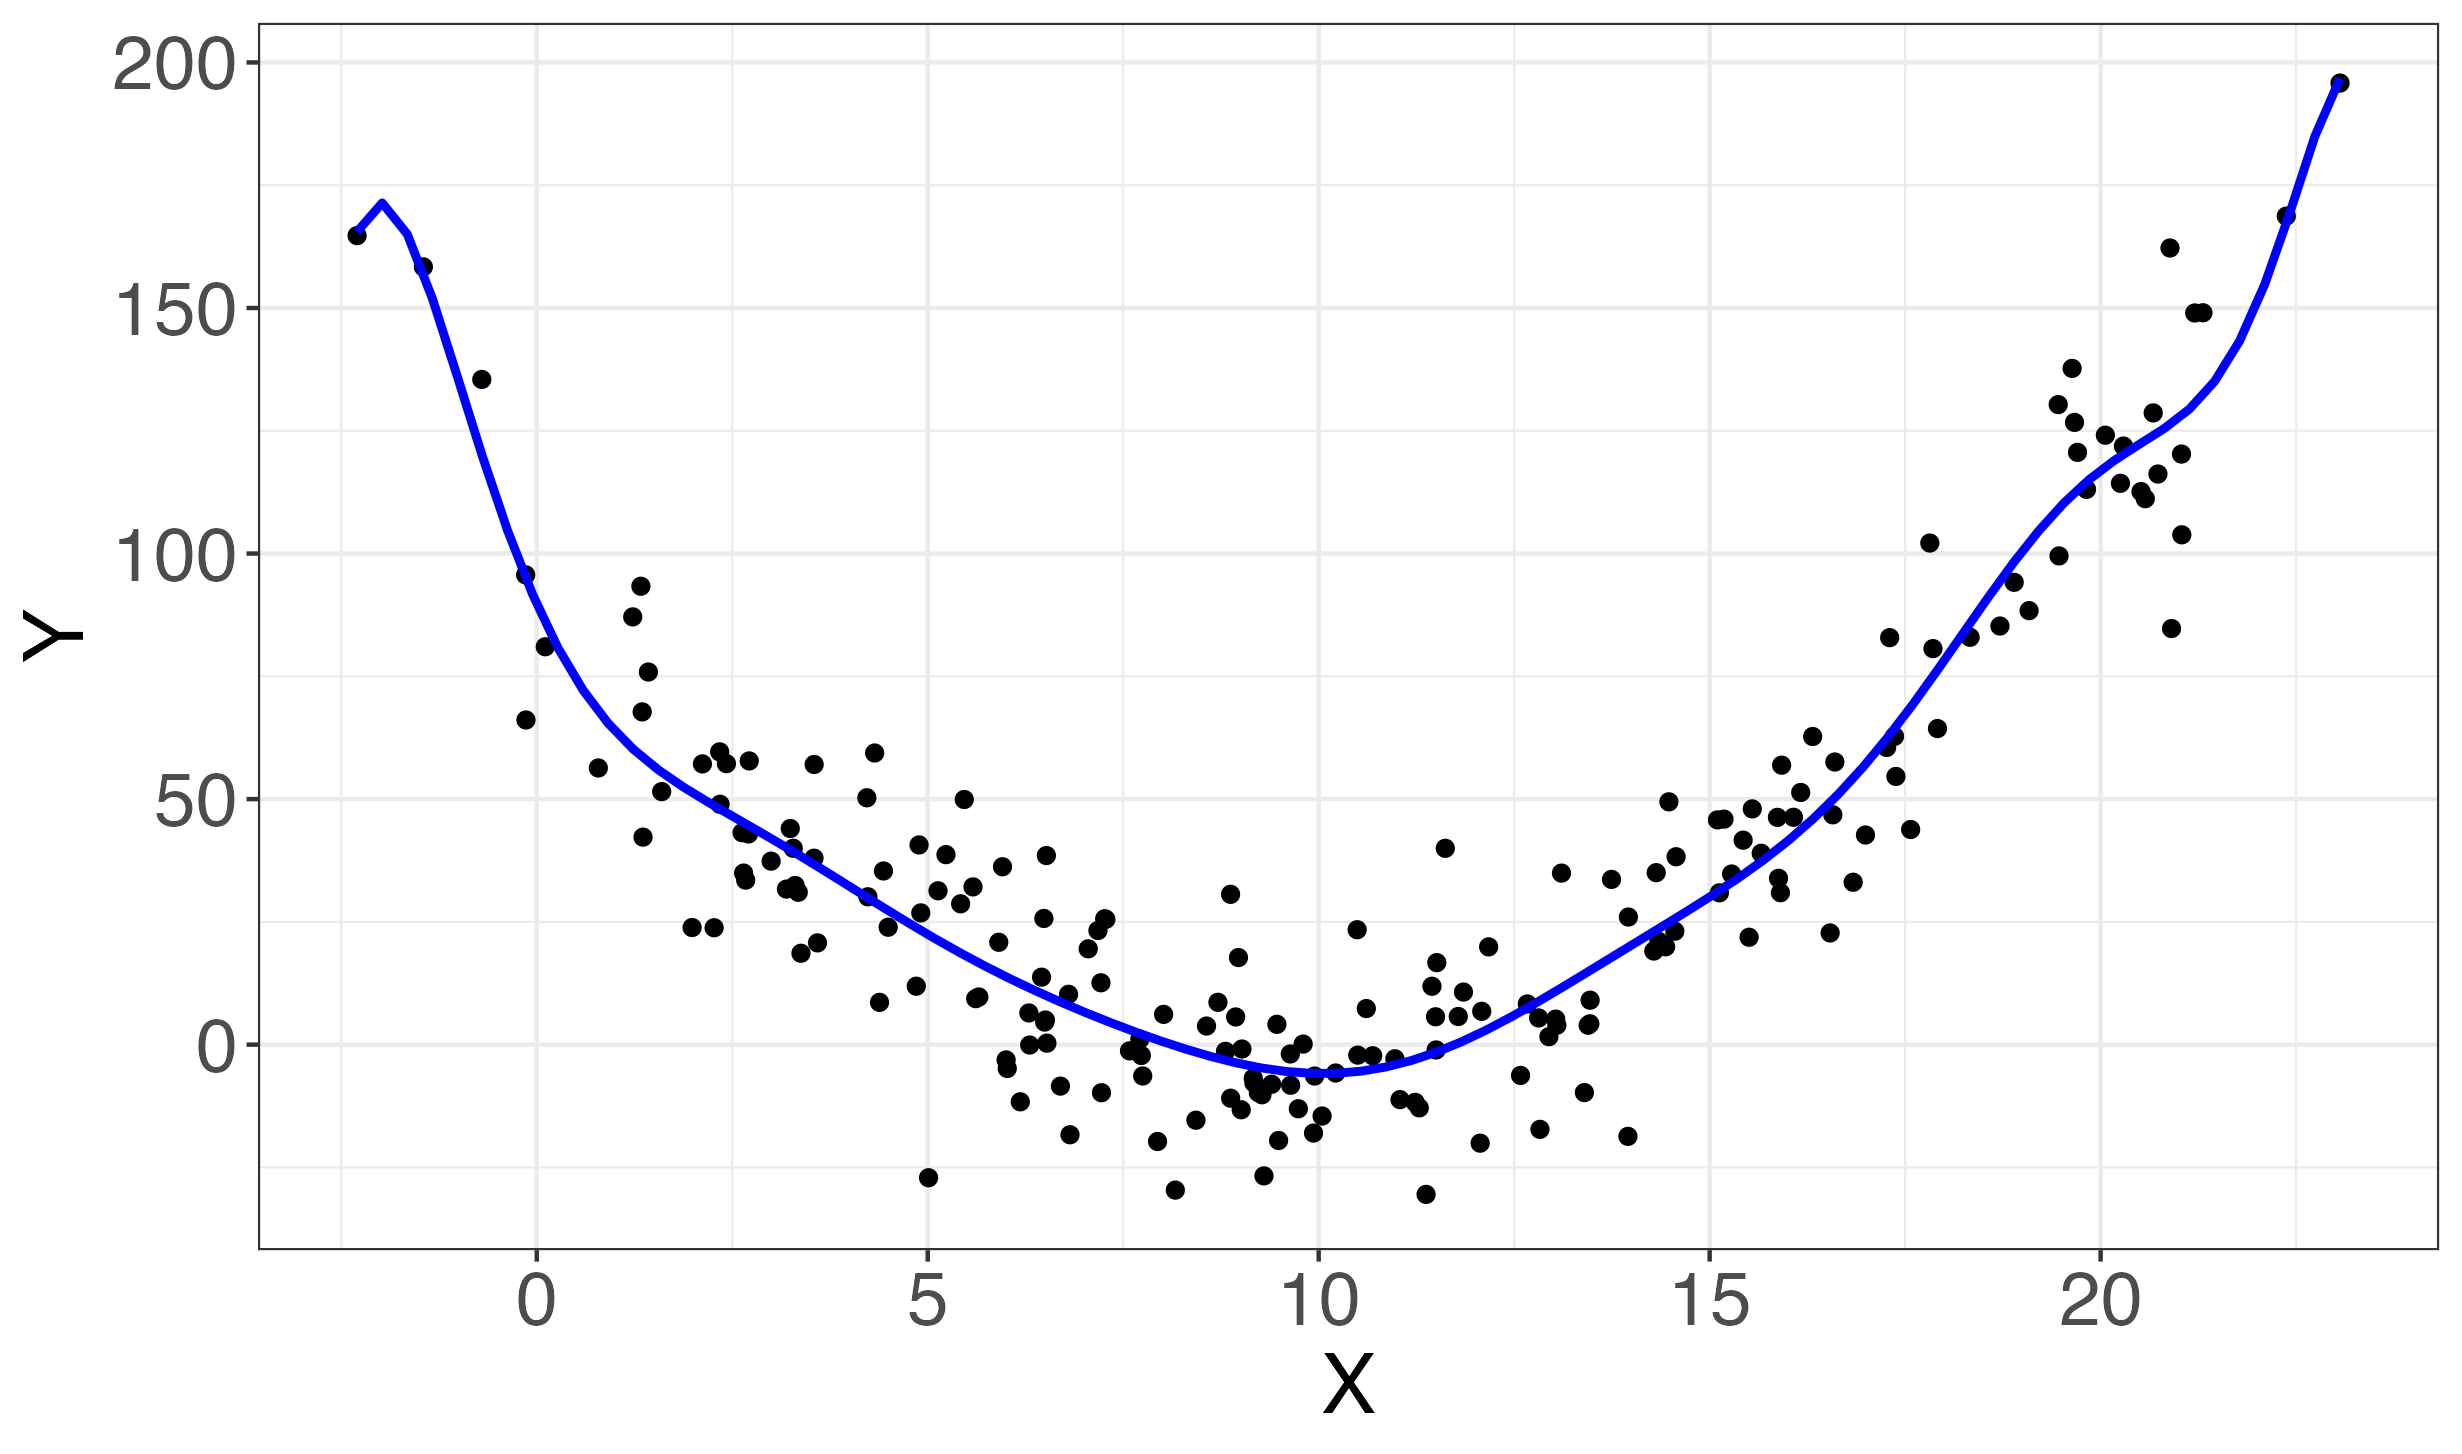
\includegraphics[scale=0.4]{figures/overfit4.png}

\end{frame}

\begin{frame}{Overfitting: Example}
OR we could \textcolor{orange}{interpolate} to get perfect predictions for all of our observed data\dots

\vspace{0.3cm}

\begin{center}
	 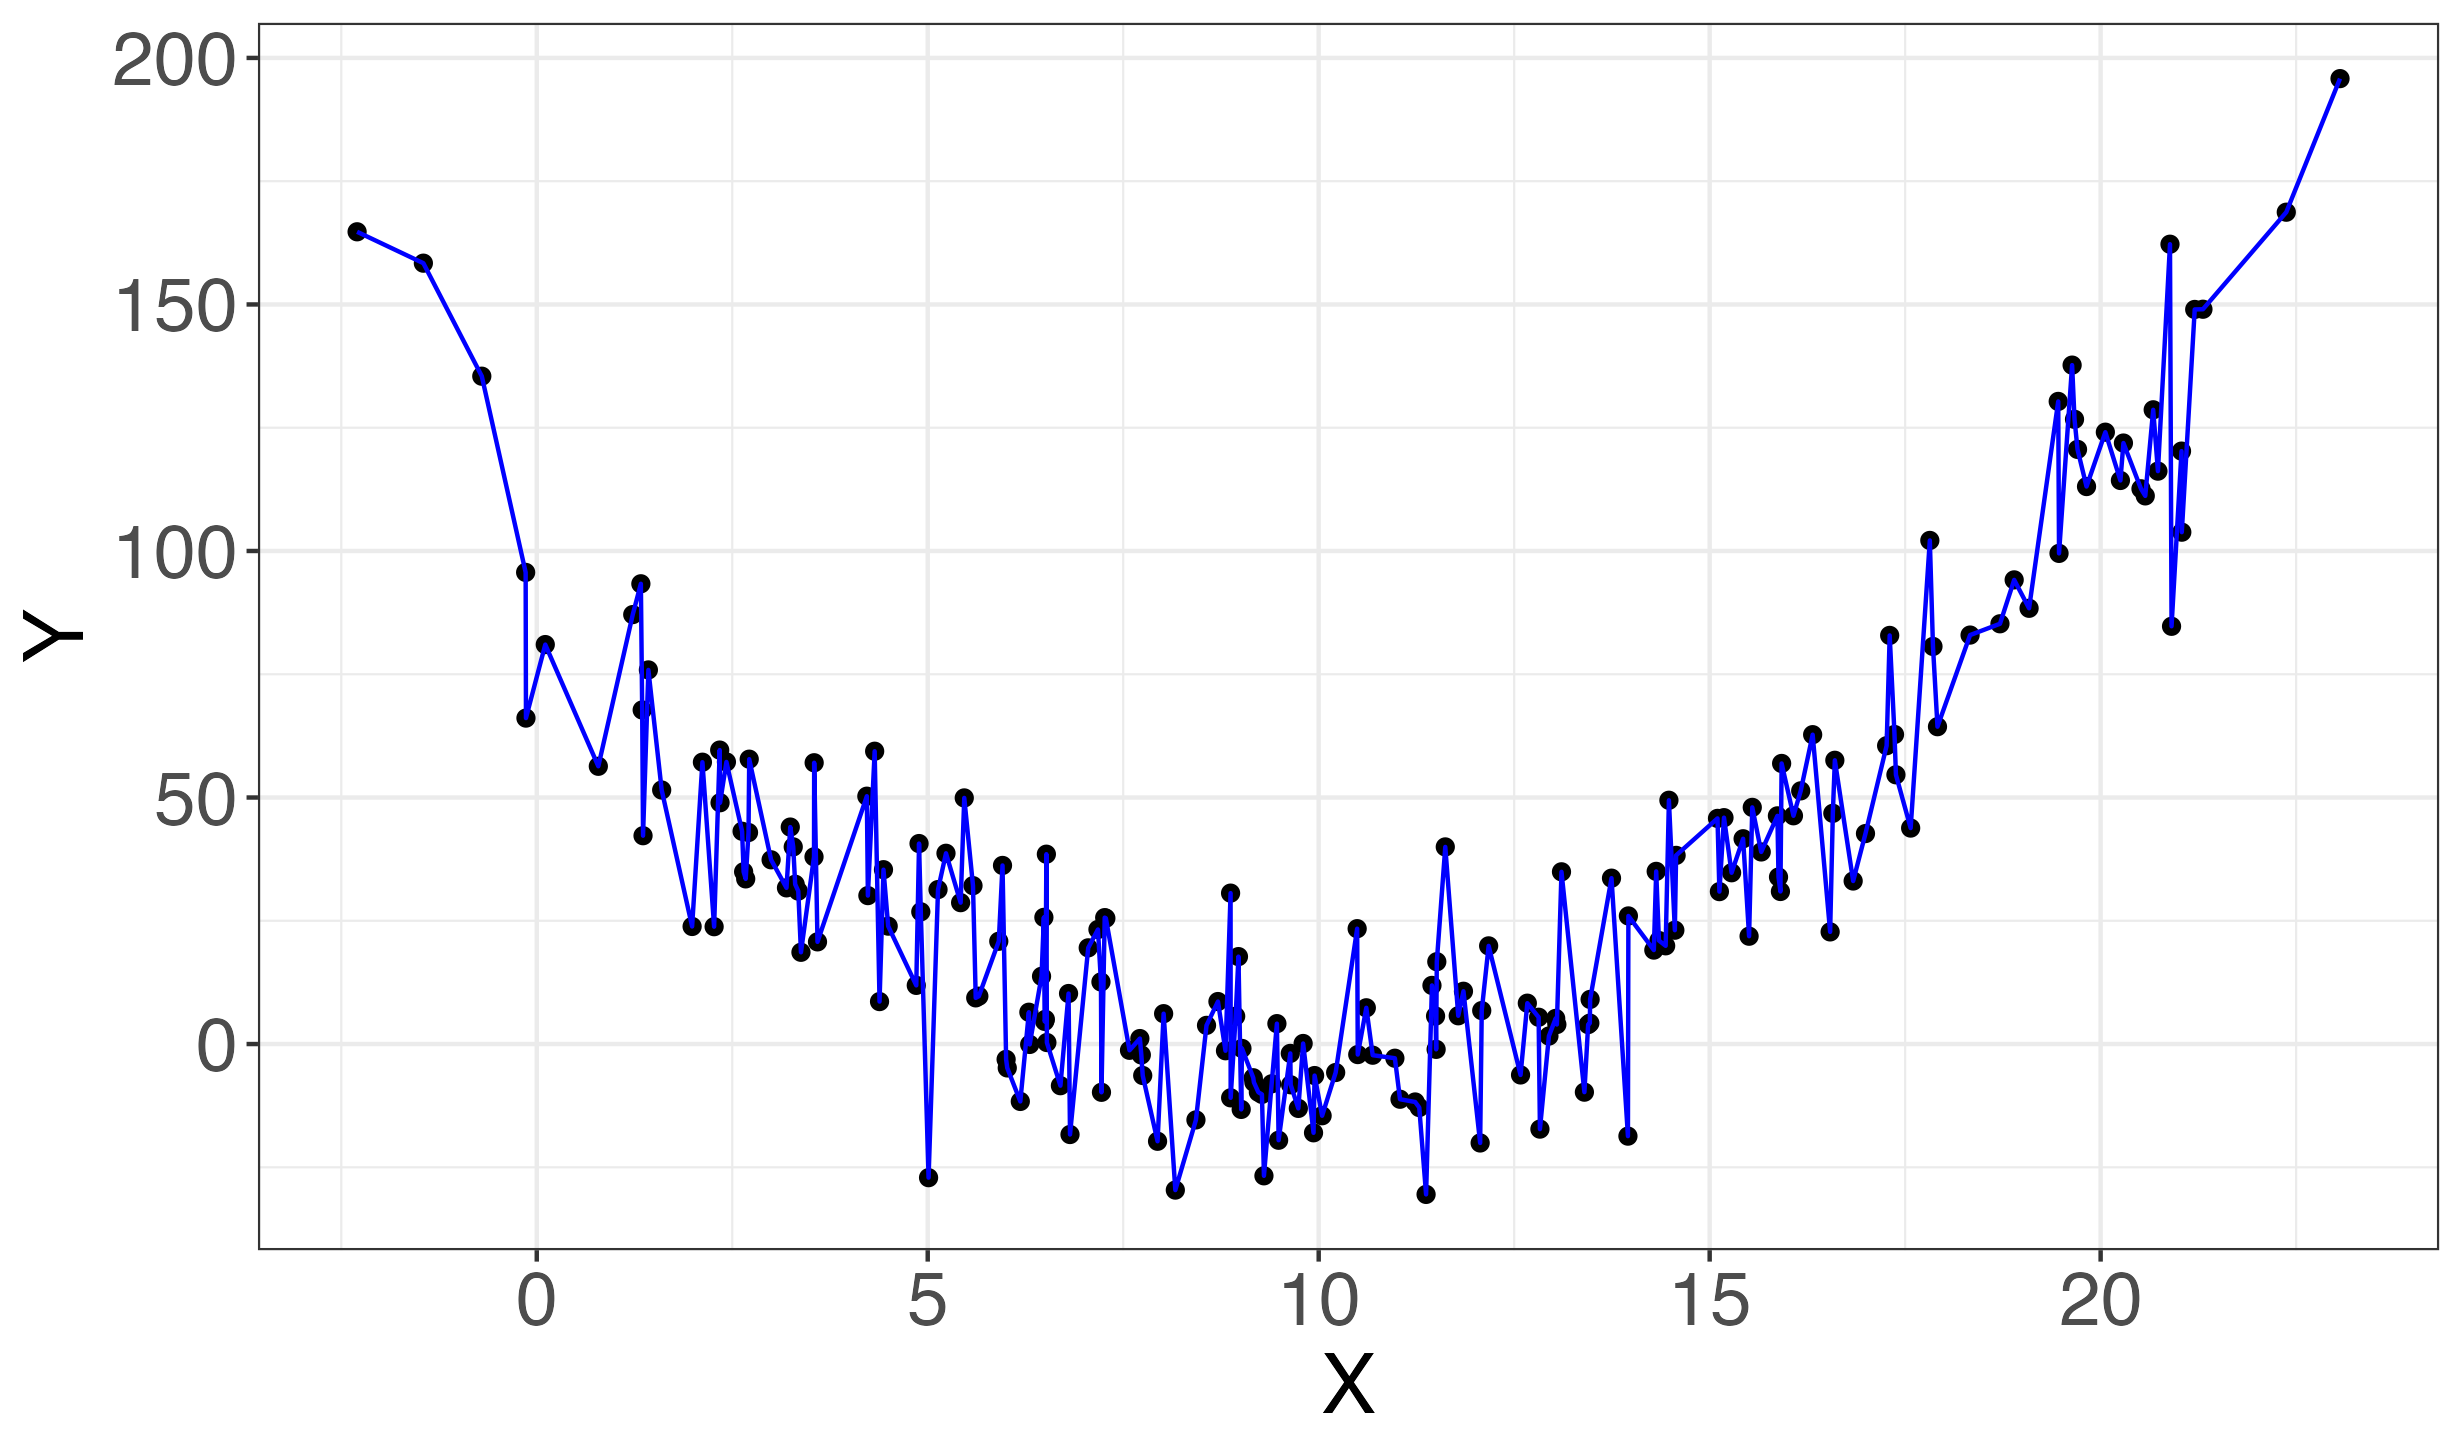
\includegraphics[scale=0.4]{figures/overfit5.png}
\end{center}
\begin{footnotesize}
	\vspace{-0.1cm}
(This should show you why evaluating our model on our training data is a bad idea!)
\end{footnotesize}
\end{frame}

\begin{frame}{Overfitting Example}
For each of these cases (other than interpolation) and extending to additional polynomials, we can fit a linear regression model and get adjusted and multiple $R^2$ values.

\vspace{0.3cm}

\begin{table}
	\begin{tabular}{l|r|r}

Model & Mult. $R^2$ & Adj. $R^2$ \\
\hline
$Y \sim X$ & 0.121 & 0.117\\
\hline
$Y \sim X + X^2$ & 0.877 & 0.876\\
\hline
$Y \sim X + X^2 + \dots + X^{13}$ & 0.888 & 0.880 \\
\hline
\vdots & \vdots & \vdots \\
\hline
$Y \sim X + X^2 + \dots + X^{15}$ & 0.8897 & \textcolor{blue}{0.8814} \\
\hline
$Y \sim X + X^2 + \dots + X^{15} + X^{16}$ & \textcolor{blue}{0.8898} & 0.8808
\end{tabular}
\end{table}

\vspace{0.3cm} At a certain point, adjusted $R^2$ decreases with the inclusion of an additional covariate in the model (in this example, $X^{16}$), while multiple $R^2$ continues to increase.
	
\end{frame}

\begin{frame}{Overfitting: Why does it matter?}
	\vspace{-0.6cm}
	
	\begin{itemize}
\item We are most concerned with how accurate our prediction model is at predicting  \textcolor{blue}{new} observations 

\medskip

		\item When we include too many covariates in our model, we run the risk of making worse predictions for new data

\end{itemize}

\vspace{0.3cm}

\textcolor{orange}{Rule of thumb:} If two models differing by a single covariate have $R^2$ values that are very similar (within 0.01 of each other), it is reasonable to choose the model with fewer covariates, for the purposes of this course.
\end{frame}

\begin{frame}{$R^2$: Example in \texttt{R}}
Suppose we are (again) interested in predicting a baby's birthweight based on birth parent's age, marital status, whether or not they smoke during pregnancy, and weight prior to pregnancy. 

\bigskip

We are interested in seeing if including the covariate indicating the birth parent drank during pregnancy improves the predictive accuracy of our model, which we will measure using adjusted $R^2$.  \texttt{R}\dots


\end{frame}

\begin{frame}[fragile]{$R^2$: Example in \texttt{R}}
	
	\vspace{-8 mm}
	
	\footnotesize
	
\begin{verbatim}
> mod <- lm(data = births, bwt ~ age + married + smoke + wpre + drink)
> summary(mod)

Call:
lm(formula = bwt ~ age + married + smoke + wpre + drink, data = births)

Residuals:
Min       1Q   Median       3Q      Max 
-3143.21  -295.64    25.88   338.16  1747.18 

Coefficients:
Estimate Std. Error t value Pr(>|t|)    
(Intercept) 2753.591     70.709  38.942  < 2e-16 ***
age            4.104      1.979   2.074 0.038197 *  
married      100.044     29.782   3.359 0.000793 ***
smoke       -210.533     44.673  -4.713 2.58e-06 ***
wpre           3.249      0.315  10.312  < 2e-16 ***
drink        -64.637    101.614  -0.636 0.524766    
---
Signif. codes:  0 ‘***’ 0.001 ‘**’ 0.01 ‘*’ 0.05 ‘.’ 0.1 ‘ ’ 1

Residual standard error: 542.4 on 2494 degrees of freedom
Multiple R-squared:  0.06169,	Adjusted R-squared:  0.05981 
F-statistic: 32.79 on 5 and 2494 DF,  p-value: < 2.2e-16
\end{verbatim}
\end{frame}

\begin{frame}[fragile]{$R^2$: Example in \texttt{R}}
	
		
	\vspace{-8 mm}
	
	
	\footnotesize
\begin{verbatim}
> mod <- lm(data = births, bwt ~ age + married + smoke + wpre)
> summary(mod)

Call:
lm(formula = bwt ~ age + married + smoke + wpre, data = births)

Residuals:
Min       1Q   Median       3Q      Max 
-3142.31  -294.47    26.18   338.30  1748.30 

Coefficients:
Estimate Std. Error t value Pr(>|t|)    
(Intercept) 2754.339     70.691  38.963  < 2e-16 ***
age            4.042      1.976   2.045 0.040979 *  
married      100.209     29.778   3.365 0.000776 ***
smoke       -212.264     44.585  -4.761 2.04e-06 ***
wpre           3.251      0.315  10.321  < 2e-16 ***
---
Signif. codes:  0 ‘***’ 0.001 ‘**’ 0.01 ‘*’ 0.05 ‘.’ 0.1 ‘ ’ 1

Residual standard error: 542.3 on 2495 degrees of freedom
Multiple R-squared:  0.06154,	Adjusted R-squared:  0.06003 
F-statistic:  40.9 on 4 and 2495 DF,  p-value: < 2.2e-16
\end{verbatim}
\end{frame}



\begin{frame}{$R^2$: Example in \texttt{R}}
The adjusted $R^2$ from the model including an additional covariate indicating whether or not birth parent drank during pregnancy is 0.05981, while for the smaller model adjusted $R^2$ is 0.06003. 

\bigskip
These values are very similar, and the larger model with the additional covariate actually has a  \textcolor{blue}{lower} adjusted $R^2$ than the smaller model. This suggests that the inclusion of a covariate for drinking will likely not improve prediction accuracy.  

\vspace{0.3cm}

\textcolor{blue}{Question:} How would we interpret the multiple $R^2$ value (0.05755) from the model containg covariates for age, marital status, smoking status, and weight prior to pregnancy?  

\vspace{0.3cm}

\textcolor{blue}{Answer:} 5.8\% of the variation in child's birthweight is explained by the variation in birth parent's age, marital status, smoking status, and weight prior to pregnancy. 

\end{frame}
% include slide about comparing multiple predictive models

\subsection{Mean Squared Error}

%\begin{frame}{Mean squared error}
%We have now seen a measure of prediction accuracy that involves only the training dataset. What can we use to quantify prediction accuracy using our observed and predicted values for our testing dataset?
%
%\vspace{0.3cm}
%
%Intuitively, we can consider quantifying accuracy based on the  \textcolor{blue}{difference} between observed and predicted values for each observation. We could then make sure that differences are treated equally regardless of sign (positive or negative), and take the average of these differences across all observations to get a single number, quantifying how far off our predictions are from the truth.  
%\end{frame}

\begin{frame}{Mean squared error}
	
\vspace{-7 mm}


\textcolor{blue}{Mean squared error (MSE):} $\frac{1}{n} \sum_{i = 1}^n (Y_i - \hat{Y}_i)^2$

\bigskip

The average of squared differences between observed outcomes $Y_i$ and predicted values $\hat{Y}_i$


\bigskip

 
The lower our MSE is, the better our predictions. Note that if $Y_i = \hat{Y}_i$ for all observations (our predicted values are the same as our observations), MSE is equal to zero.



\begin{figure}
	\centering
	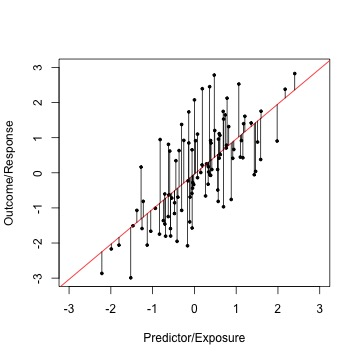
\includegraphics[scale = 0.4, trim={0 0 0 15mm},clip]{figures/linear-regr-ls}
\end{figure}

\end{frame}


\begin{frame}{MSE and Overfitting}
	There is no adjusted version of MSE. Adding more variables will always increase the MSE of the model on our observed data. 
	
	\bigskip
	
	\textcolor{blue}{Question}: So how do we prevent overfitting when using the MSE?
	
	\bigskip
	
	\textcolor{blue}{Answer}: We use training and testing datasets
	

	
\end{frame}



\subsection{Training and testing data}

\begin{frame}{Training and testing data}
	In practice, since we clearly do not have access to data that we have not yet collected, we instead pretend that some of our observed data is ``new," and we try to accurately predict the observed outcomes of those ``new" observations. This involves splitting our dataset into \textcolor{blue}{training} and \textcolor{blue}{testing} data.
	
	\vspace{0.3cm}
	
	\textcolor{blue}{Training data:} The subset of data we use for ``training" (fitting) our predictive model
	
	\vspace{0.3cm}
	
	\textcolor{blue}{Testing data:} The subset of data we use for ``testing" how accurate our predictive model is, often comparing observed outcomes to fitted values
	
	\vspace{0.3cm}
	
	It is common in practice to use a random sample of 70\% of your observations for training data, and 30\% of your observations for testing, though this can vary quite a bit!
	
	%Question: what are the pros and cons of increasing the test data set more? What are the pros and cons of increasing the training data set more?
	
\end{frame}

\begin{frame}{Training and testing data: in \texttt{R}}
	We can create training and testing datasets in \texttt{R} by taking a random sample of rows from our data \texttt{df}, using the \texttt{sample} function:
	
	\vspace{0.1cm}
	
	\begin{figure}
		\centering 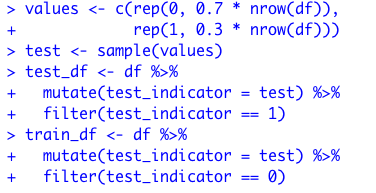
\includegraphics[scale=0.5]{figures/traintest.png}
	\end{figure}
	
	\vspace{0.1cm}
	
	We have now created two separate datasets, \texttt{test\_df} and \texttt{train\_df}, by randomly splitting our dataset into two groups, with 70\% of observations in the training dataset and 30\% in the testing dataset.
	
	% break down what this is doing during class
\end{frame}

\begin{frame}{Training and testing data: in \texttt{R}}
	We then use the training data to fit our model, and obtain predictions for the testing data:
	
	\vspace{0.3cm}
	
	\texttt{mod <- lm(data = train\_df, ...)} \\
	\texttt{predictions <- predict(mod, newdata = test\_df)}
	
	\vspace{0.3cm}  
	
	It might also be useful to create a new object containing the observed outcomes for individuals in the testing data:
	
	\vspace{0.3cm}
	
	\texttt{observations <- test\_df \%>\% pull(outcome variable)}
	
\end{frame}

\begin{frame}{MSE with training and testing data: Example in \texttt{R}}
	Suppose we are (again) interested in predicting a baby's birthweight based on birth parent's age, marital status, whether or not they smoke during pregnancy, and weight prior to pregnancy. We:
	\medskip
	
	\begin{enumerate}
		\item Split the data into training and testing
		\medskip
		\item Fit the model using the training data
		\medskip
		\item Use the model to predict the birth weights of the testing data
		\medskip
		\item Calculate the MSE of the testing data
	\end{enumerate}
	\bigskip
	
		\bigskip
	\textcolor{violet}{Pollev:} How can we prevent overfitting when using $R^2$?
	\scriptsize{\url{https://PollEv.com/multiple_choice_polls/p6sigPanaQ6SjcR2Yfiyg/respond}}\pause
	\medskip
	\normalsize
	
	\textcolor{blue}{Using the adjusted $R^2$}

	\end{frame}
	
\begin{frame}[fragile]{MSE with training and testing data: Example in \texttt{R}}
	
	\vspace{-7mm}
	
\begin{verbatim}
values <- c(rep(0, 0.7*nrow(births)),
rep(1,0.3*nrow(births)))

test <- sample(values)

test_data <- births %>% mutate(test_yes = test) %>%
filter(test_yes == 1)

train_data <- births %>% mutate(test_yes = test) %>%
filter(test_yes == 0)

mod <- lm(data = train_data, bwt ~ age + married + smoke + wpre)

predictions <- predict(mod, newdata = test_data)
observations <- test_data %>% pull(bwt)

mse <- mean((observations - predictions)^2)
mse
[1] 296008.3
\end{verbatim}
\end{frame}

\begin{frame}{Qualitative Assessment: Example in \texttt{R}}
	\vspace{-5 mm}
	
	We can also evaluate our model qualitatively by plotting our observed values versus our predicted values.
	
	\vspace{0.3cm}
	
	\centering 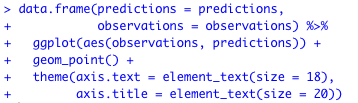
\includegraphics[scale=0.5]{figures/predict_vs_obs_code.png} \vspace{0.1cm}
	
	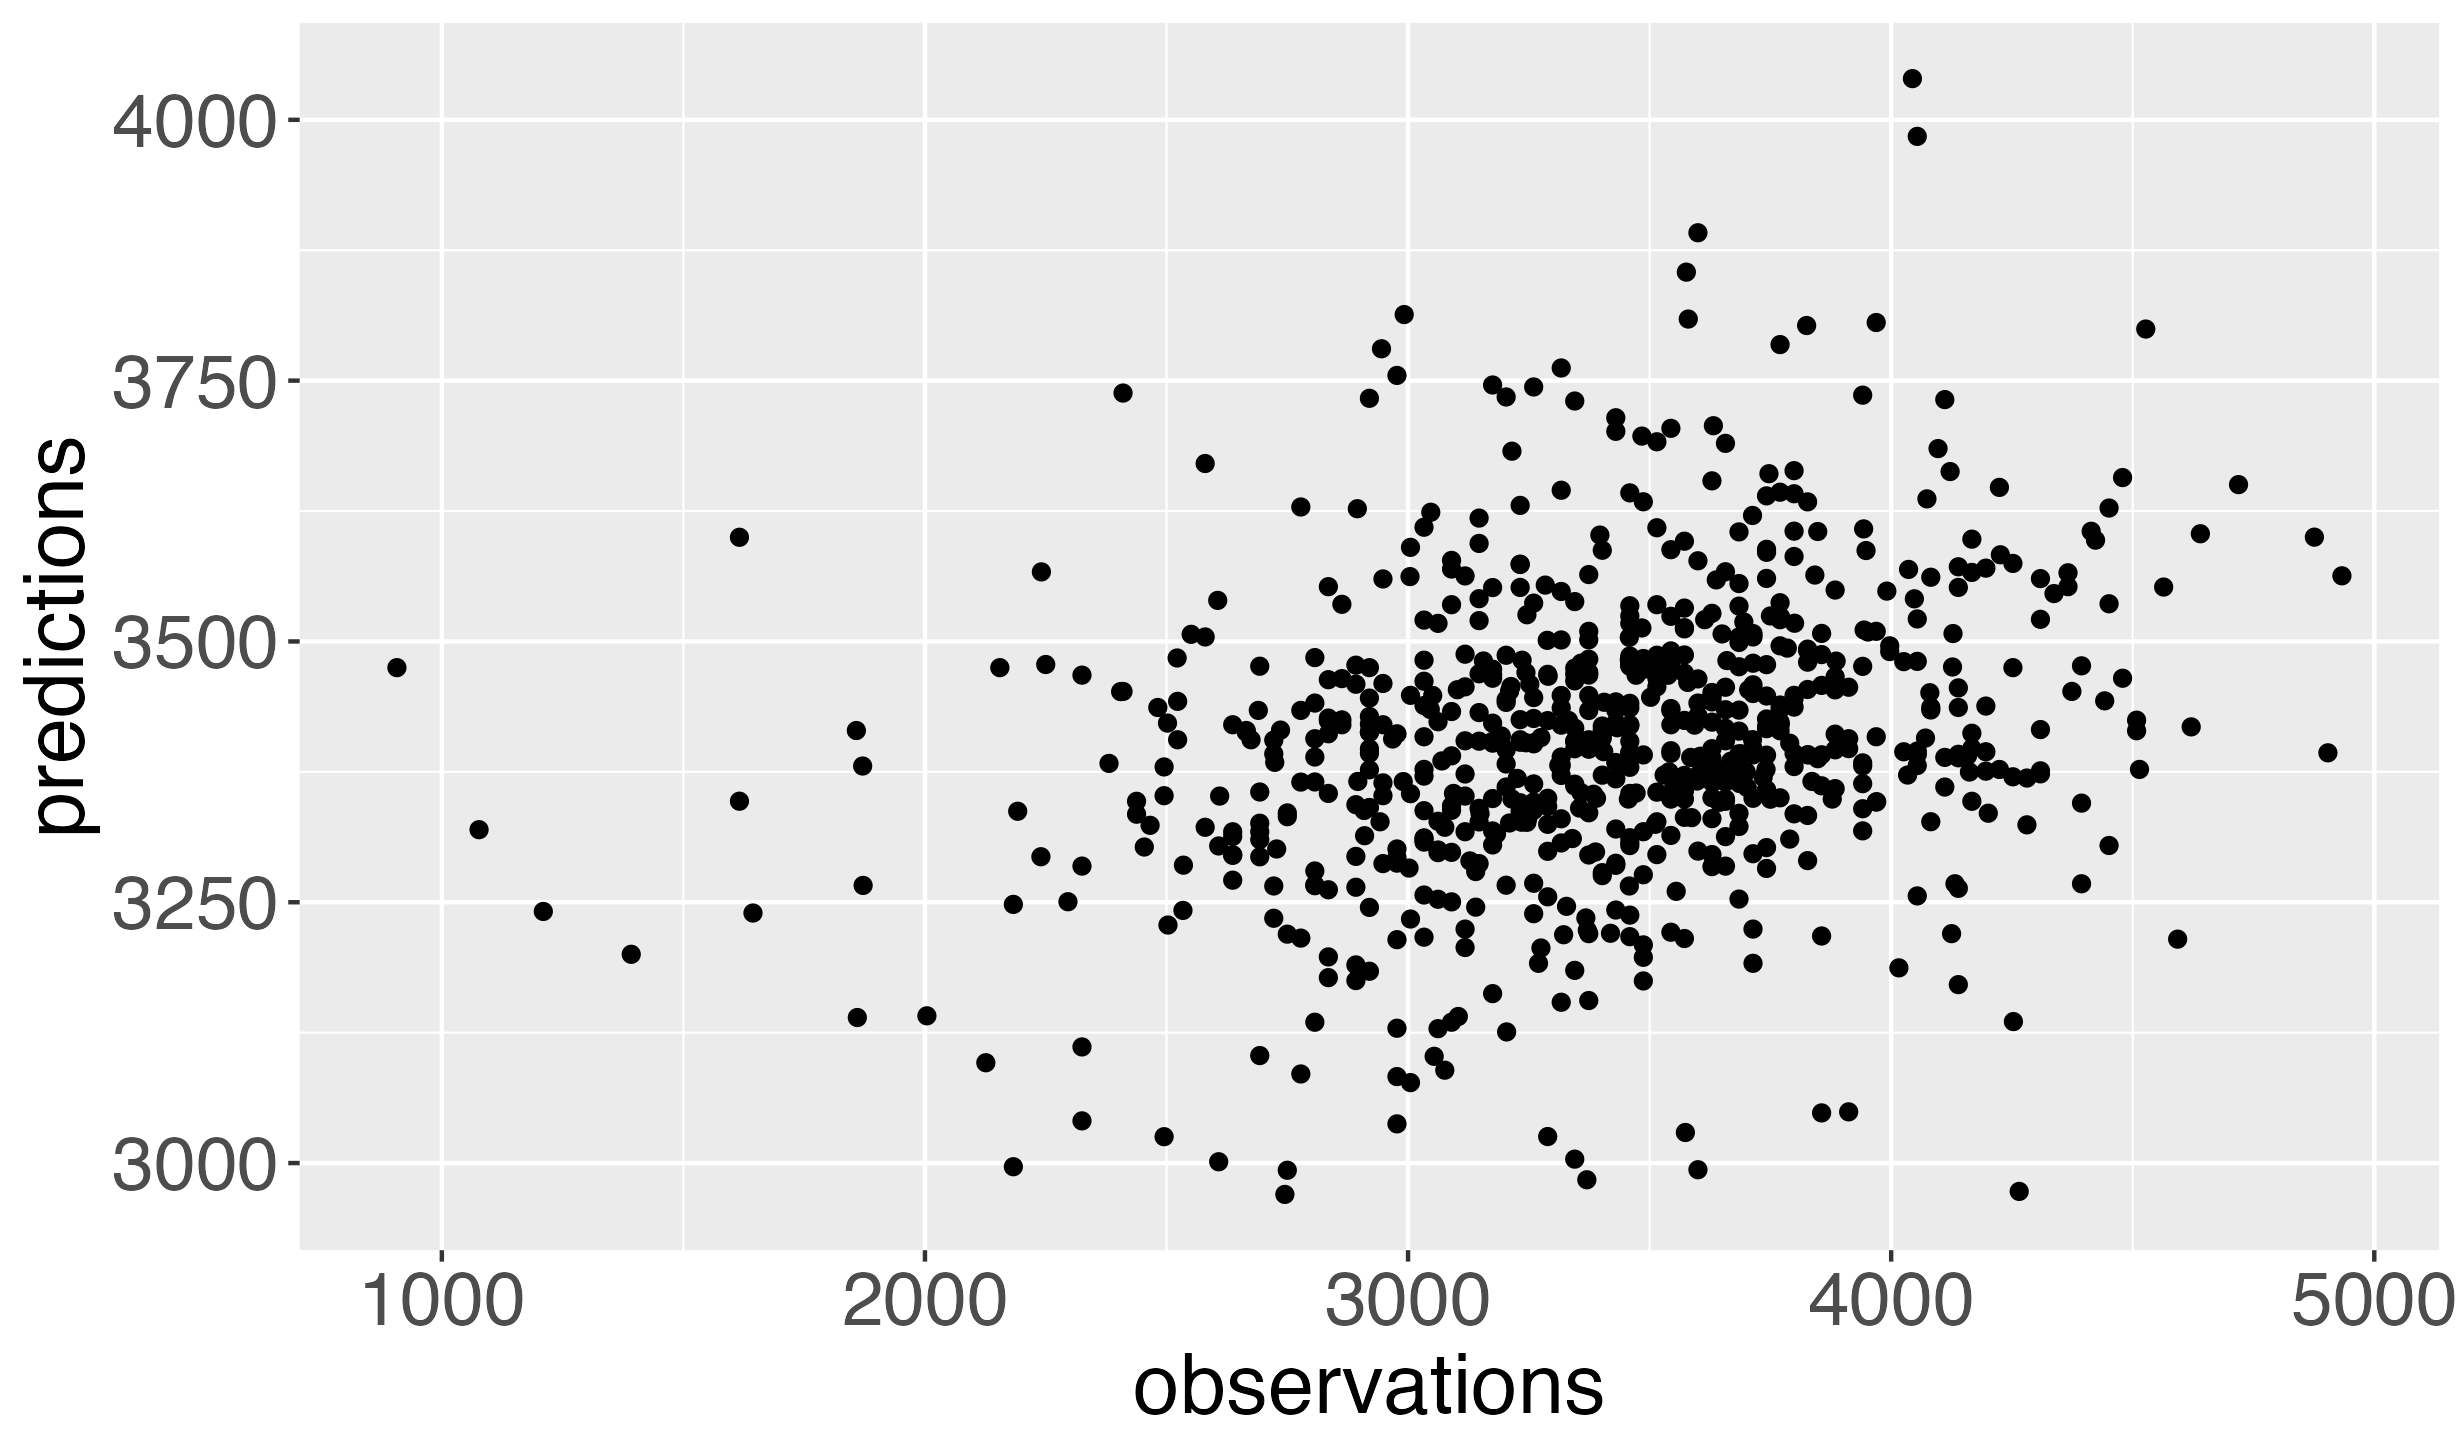
\includegraphics[scale=0.35]{figures/predict_vs_obs.png}
	
\end{frame}

\begin{frame}{Qualitative Assessment: Example in \texttt{R}}
	\vspace{-0.6cm}
	\begin{figure}
		\centering 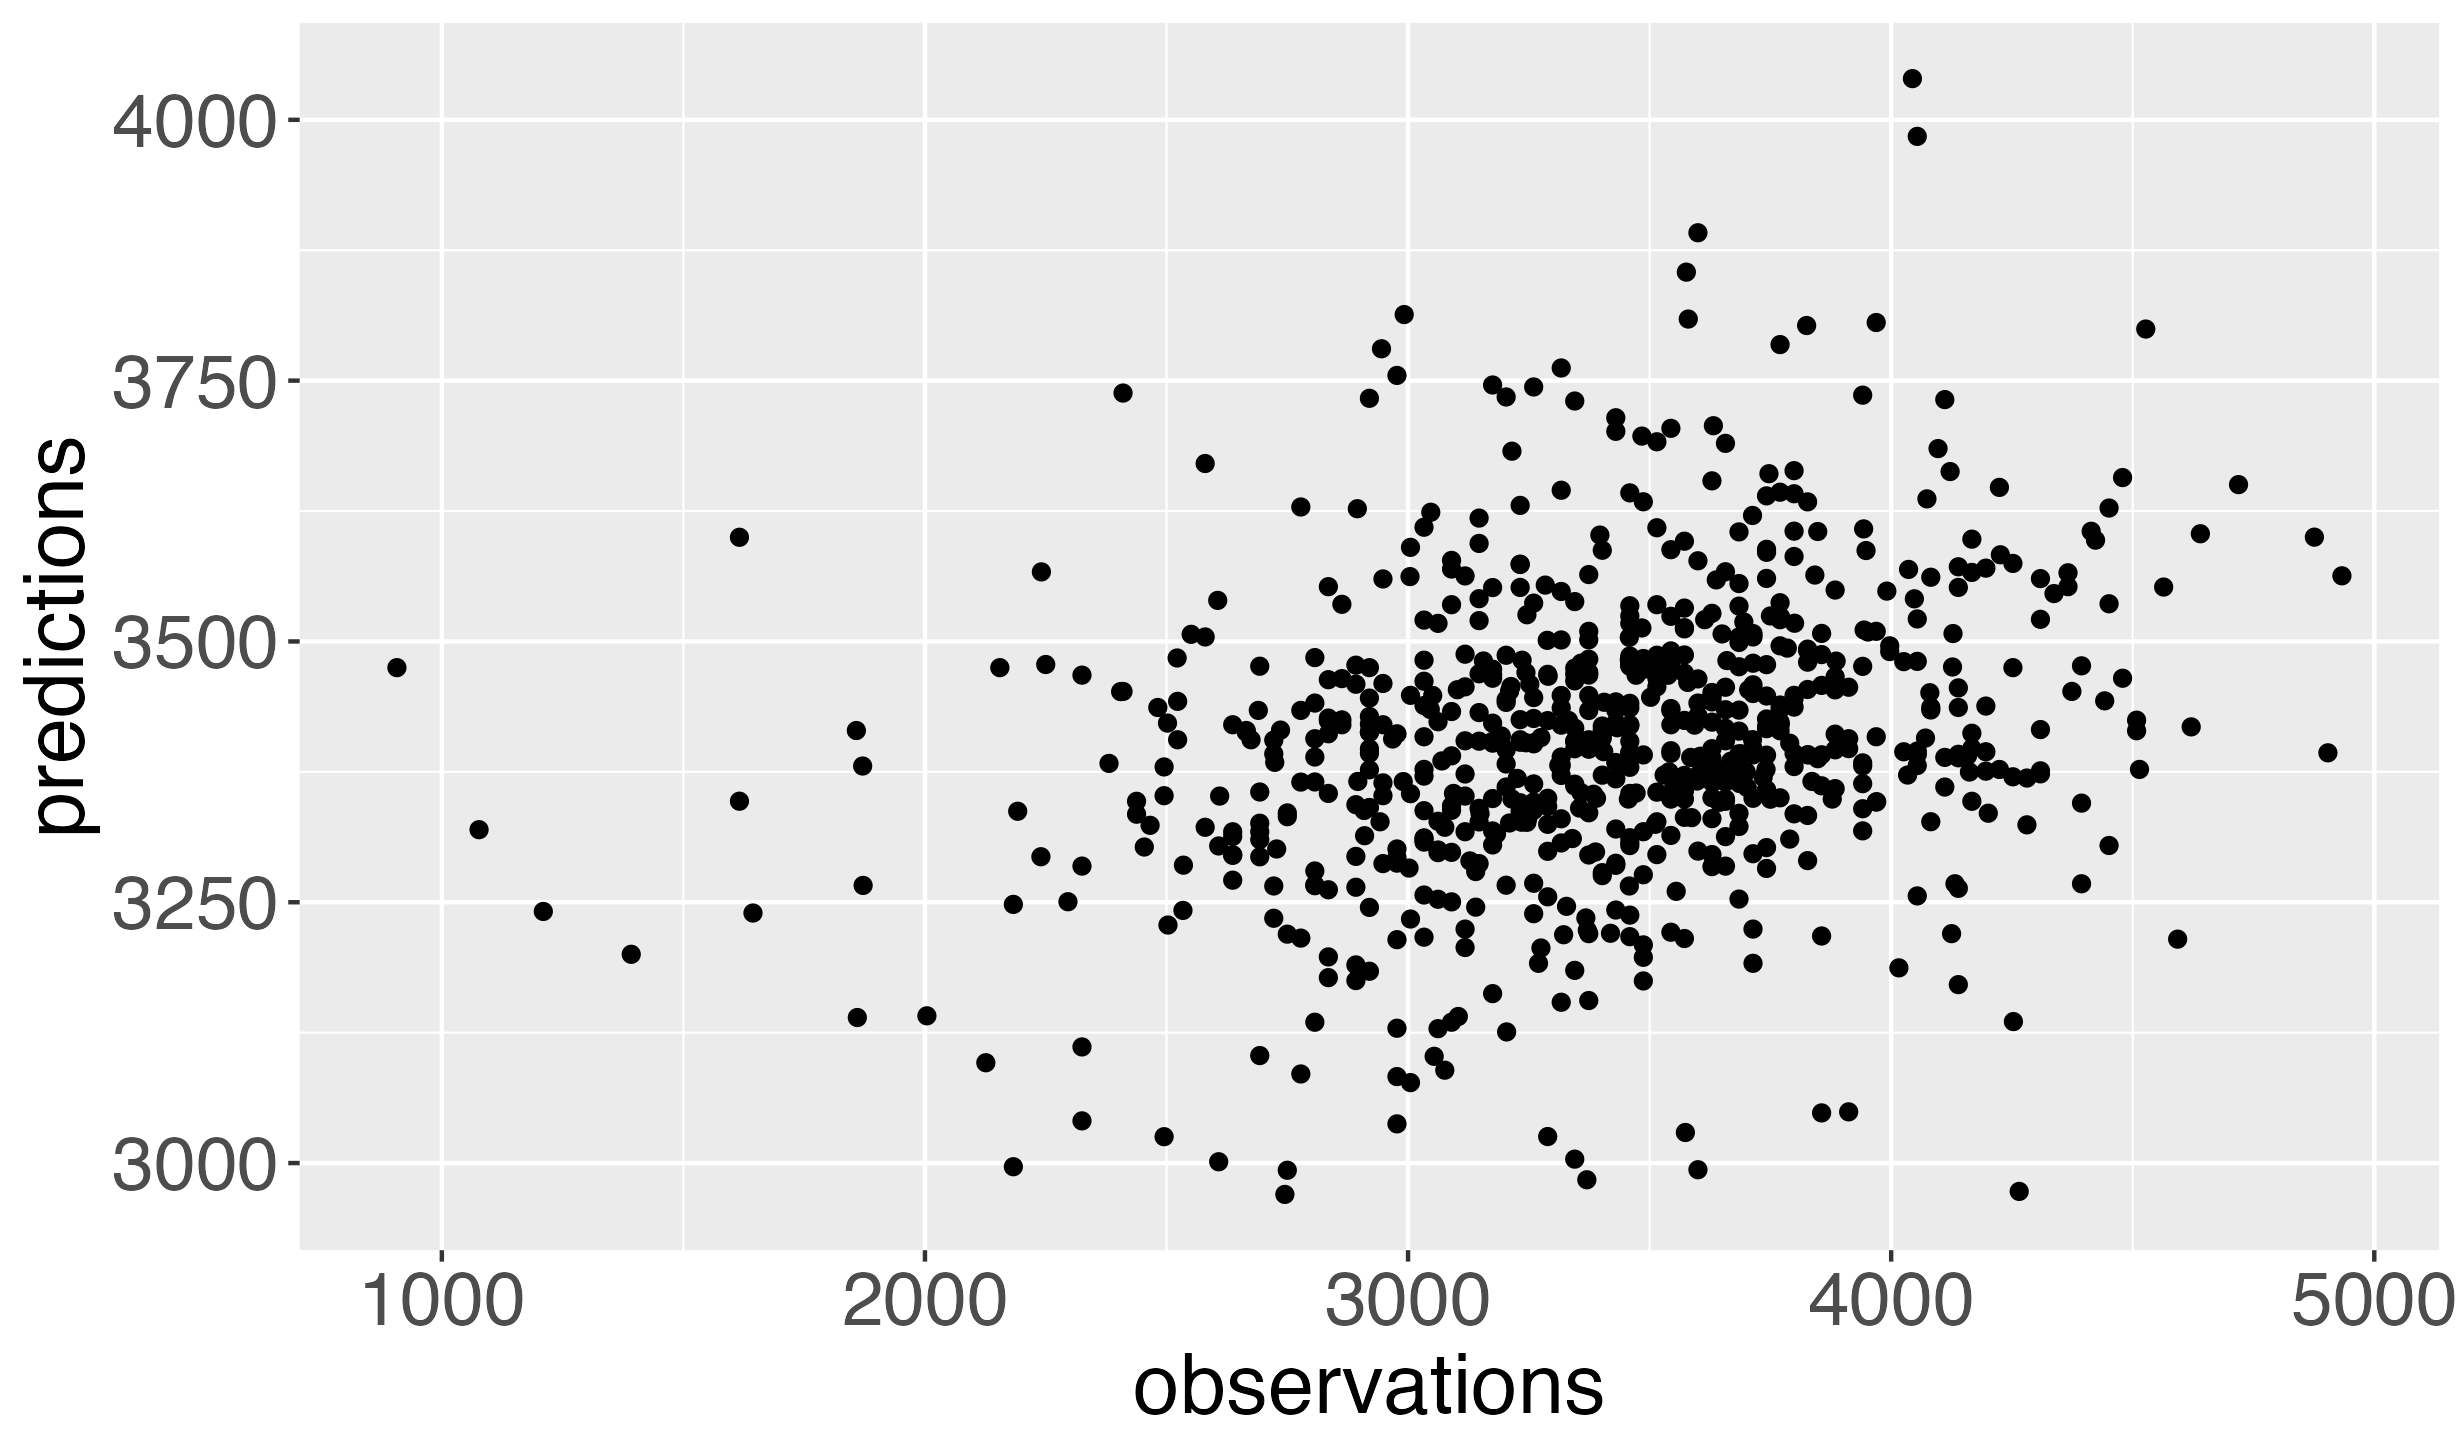
\includegraphics[scale=0.3]{figures/predict_vs_obs.png}
	\end{figure}
	
	\textcolor{blue}{Question:} What would our scatterplot comparing observed outcomes and predictions look like if we were able to  \textcolor{blue}{perfectly} predict the observed outcome?  
	
	\vspace{0.3cm}
	
	\textcolor{blue}{Answer:} If we perfectly predicted the observed outcome, we would have predictions = observations (which corresponds to the line $y = x$). All of our points would lie on the line $y = x$ in our scatterplot!
	
\end{frame}

\begin{frame}{Qualitative Assessment: Example in \texttt{R}}
	\vspace{-5 mm}
	
	We can overlay a line with slope equal to 1 and intercept 0 on our scatterplot to see how well the points fall on the line:
	
	\vspace{0.3cm}
	
	\centering 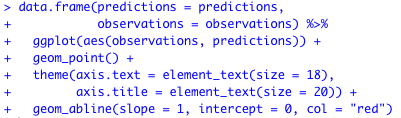
\includegraphics[scale=0.45]{figures/predict_vs_obs_code2.png} \vspace{0.1cm}
	
	\begin{figure}
		\centering 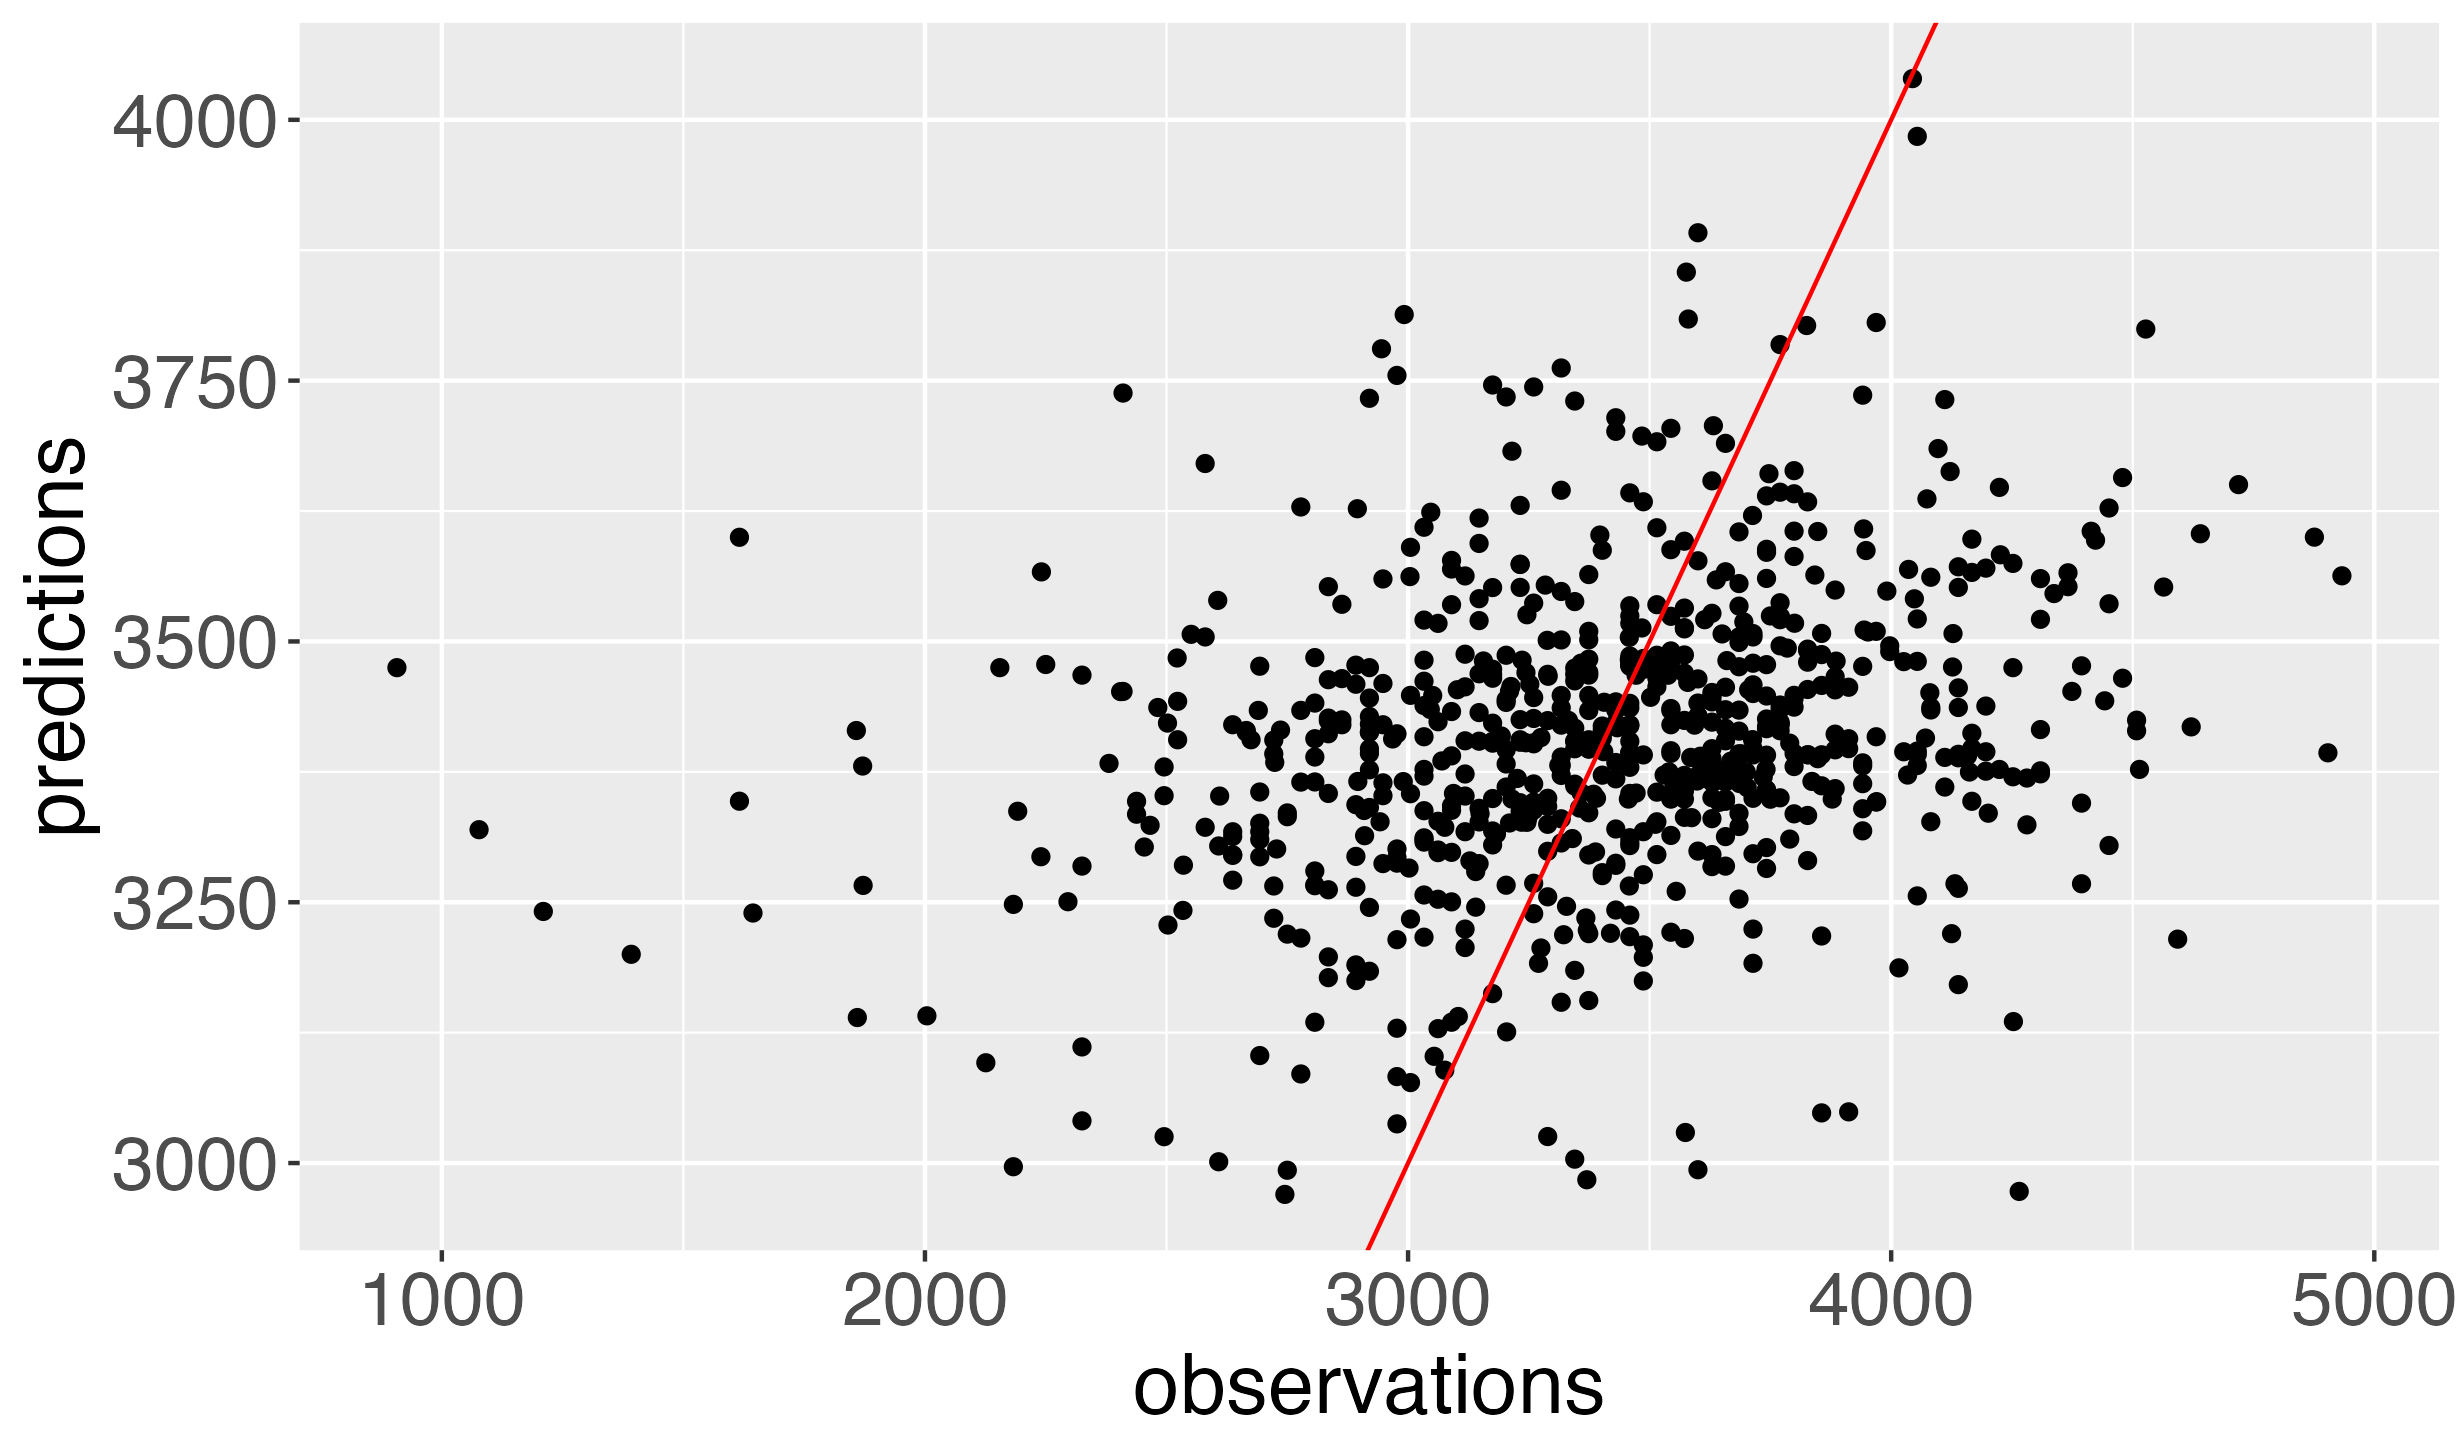
\includegraphics[scale=0.35]{figures/predict_vs_obs2.png}
	\end{figure}
	
\end{frame}




\begin{frame}{Cross-validation 
\includegraphics[scale=0.01]{figures/technical.png} }
	\vspace{-5 mm}
	
	So far we have only discussed creating a  \textcolor{blue}{single} testing and training dataset from our original dataset. This is sometimes done in practice, and is completely justifiable! 
	
		\vspace{0.3cm}
	
	However, it also common to instead split our original dataset into training and testing datasets  \textcolor{blue}{multiple} times, and compute an average measure of prediction accuracy across these multiple training and testing datasets.
	
	\vspace{0.3cm}
	
	\textcolor{blue}{Cross-validation:} The process of creating training and testing datasets many times, over which we compute measures of prediction accuracy. These measures are then averaged to assess predictive model performance.
	
	\vspace{0.3cm}
	
	What? By creating many training and testing datasets from the model and averaging across them, \textcolor{blue}{cross-validation reduces the variability in our prediction accuracy measures}, and therefore gives us a more precise measure of prediction accuracy.
	
\end{frame}



\begin{frame}{Cross-validation 
\includegraphics[scale=0.01]{figures/technical.png} }
	What does this look like in practice?
	
	\vspace{0.3cm}
	
	for $j = 1, \dots, k$ times:
	
	\vspace{0.3cm}
	
	\begin{enumerate}
		\item Randomly split the dataset into training (\texttt{train\_df\_j}) and testing (\texttt{test\_df\_j}) data
		\item Fit our model (\texttt{mod\_j}) on the training data set
		\item Obtain predictions (\texttt{predictions\_j}) using the testing dataset 
		\item Compute MSE (\texttt{mse\_j}), or other measures of prediction accuracy, using predictions and observations 
	\end{enumerate}
	
	\vspace{0.3cm}
	
	and compute the average MSE across all testing datasets as $\frac{1}{k} \sum_{i = 1}^k \text{MSE}_j$ 
	
\end{frame}


% is it okay to fit multiple models? yes because prediction not inference
\begin{frame}{How many models can we make?}
	\vspace{-0.5cm}
	You may have heard of \textcolor{orange}{data dredging} or \textcolor{orange}{p-hacking} before, which involves misusing either data selection mechanisms or statistical analyses in order to seek out statistically significant results.
	
	\vspace{0.3cm}
	
	
\includegraphics[scale=0.01]{figures/technical.png} In these scenarios, researchers often fit  \textcolor{blue}{many} statistical models to their data in an attempt to find a p-value less than 0.05. The problem with this is that when you perform multiple statistical analyses (multiple hypothesis tests), Type I error rate (the probability that we reject the null hypothesis even though the null is true) can get very large. 
	
	\vspace{0.3cm}
	
	With prediction, we are not conducting hypothesis tests. We are simply trying to find the ``best" predictive model using the data that we have access to. 
	
	\vspace{0.3cm}
	
	With prediction, we can use the test dataset to make sure we aren't ``cheating" in building our models. As long as we don't look at the test dataset until the end, \textcolor{blue}{we can fit as many models as we want!}
	
\end{frame}

\subsection{Bias-variance tradeoff}

\begin{frame}{Bias-variance tradeoff }
	With any prediction model we fit, we will have measures of \textcolor{blue}{bias} and \textcolor{blue}{variance}.
	
	\vspace{0.3cm}
	
	\begin{itemize}
		\item \textcolor{blue}{Bias:} how far our predictions are from the truth, on average
		\item \textcolor{blue}{Variance:} how variable our predictions are
	\end{itemize}
	
	\vspace{0.3cm} 
	
	Both bias and variance have mathematical expressions (not included here), that lead us to the equation
	$$
	\text{MSE} = \text{Bias}^2 + \text{Variance}
	$$  
	
	In many prediction scenarios (as we saw), we want a predictive model that  \textcolor{blue}{minimizes} MSE. Ideally then, we want a model where both bias and variance are small. 
\end{frame}

\begin{frame}{Bias-variance tradeoff}
	\vspace{-0.4cm}
	Note that we could have two different models that produce predictions with the same MSE, but have very different values for bias and variance:
	
	\vspace{0.3cm}
	
	\begin{itemize}
		\item MSE = $10^2 + 1 = 101$ (Bias = 10, Variance = 1)
		\item MSE = $1^2 + 100 = 101$ (Bias = 1, Variance = 100)
	\end{itemize}
	
	\vspace{0.3cm}
	
	 When improving upon a prediction model (making a new model with better predictive accuracy), we often have to choose between minimizing bias  \textcolor{blue}{or} minimizing variance.  This is called the \textcolor{orange}{bias-variance tradeoff}. 
	
	\vspace{0.3cm}
	
	\small In certain scenarios, we may be okay with our predictions having a larger amount of bias in exchange for smaller variances. In some scenarios, we may require  \textcolor{blue}{no} bias, and therefore only focus on minimizing variance in our predictions. This will depend on the context of the prediction problem!
\end{frame}

\begin{frame}{Bias-variance tradeoff}
	\vspace{-5 mm}
	
	In general:
	\bigskip
	
	More complex models:
	\medskip
	\begin{itemize}
		\item will have \textcolor{blue}{less} bias
		\medskip
		\item will have \textcolor{violet}{more} variance
	\end{itemize}
	\bigskip
	
	Less complex models:
	\medskip
	\begin{itemize}
		\item will have \textcolor{blue}{more} bias
		\medskip
		\item will have \textcolor{violet}{less} variance
	\end{itemize}
	\medskip
	
	\textcolor{violet}{Pollev:}{ When we overfit a model, is the issue that we have too much variance or that we have too much bias?}
	\scriptsize{\url{https://PollEv.com/multiple_choice_polls/5wEfYaYo78SVMNGMAJEkl/respond}}\pause
	\medskip
	
	\normalsize
	\textcolor{blue}{too much variance}


\end{frame}



\section{Considerations besides accuracy}

\begin{frame}{Considerations besides accuracy}
	\textcolor{blue}{Interpretability}
	\medskip
	\begin{itemize}
	\item When models are used in high-risk situations such as health care, we might find it very important to \textcolor{blue}{understand} how the model works
	\medskip
	\item In order to assess whether the decision making process is appropriate
	\medskip
	\item this is fairly easy with linear regression, but can be difficult with more complex prediction models 
	\end{itemize}
	
\end{frame}

\begin{frame}{Considerations besides accuracy}
	\vspace{-5 mm}
	
	\textcolor{blue}{Fairness}
	\medskip
	\begin{itemize}
		\item Models may be accurate according to the data but show biases based on race, gender, socioeconomic status, etc.
		\medskip
		\item Caused by biases in the data used to train the model
		\medskip
		\item Can happen even if variables for race, gender, etc aren't in the model
	\end{itemize}
\medskip

Example: Algorithm for access to health care management programs
\medskip

\begin{itemize}
	\item predicts risk of poor health
	\medskip
	\item uses health care costs to determine poor health
	\medskip
	
	\item due to structural inequities in health care, care for patients who are Black costs less
	\medskip
	
	\item predicts patients who are Black will be less sick than they are, which prevents access to health care management programs
\end{itemize}
\bigskip

\scriptsize{\url{https://publichealth.berkeley.edu/news-media/school-news/widely-used-health-care-prediction-algorithm-biased-against-black-people/}}


	
\end{frame}


\begin{frame}{Prediction in Linear Regression: Summary}
By now, you should be able to\dots

\vspace{0.3cm}
\begin{itemize}
	\item Understand and explain the difference between the scientific goals of prediction vs. inference
	\item Be able to compute fitted values in \texttt{R} and by hand
	\item Understand the importance of training vs. testing data, and how to create training and testing datasets in \texttt{R}
	\item Determine the predictive accuracy of a linear regression analysis using $R^2$ and mean squared error (MSE)
	\item Use $R^2$ and MSE to choose a prediction model
\end{itemize}
\end{frame}


%tbd


\begin{frame}[c]
\centering \huge Any Questions?
\end{frame}

\end{document}